\chapter{Supersymmetry: as an extension of Standard Model}
%\label{:Supersymmetry}
\minitoc


%It has been more than two thousand years, as thinking population of the Earth we wondered about our surroundings. We thought about what are the fundamentals of all matter around us. Our steps, starting from the first atomic theory by Democritus ($\sim 400$ B.C.) later with the better understanding of Quantum theory in the $20^{th}$ century, lead us up to Standard Model of particle physics.

%The Standard Model describes the interactions of particle and the fundamental forces driving those interactions. One of the milestones in this path is the unification of electric and magnetic forces into a single theory of electromagnetism described by Maxwell$\textquotesingle$s equations in the middle of the $19^{th}$ century. 
%The first half of the following century was a rush of particle discoveries and corresponding theories describing their natures. In this journey, the extra ordinary studies of M. Plank, E. Rutherford, A. Einstein, L. de Broglie, W. Pauli, E. Schroedinger, W.  Heisenberg, P. Dirac, E. Fermi, H. Yukawa, C.N. Yang, R. Mills and J. Schwinger were the pillars of the Standard Model, which unifies the three of the four known forces of our universe. These three forces are the electromagnetic, the weak and the strong forces. The missing fourth force is the gravity that failed to enter the SM framework. In addition to this the SM has several other shortcomings. This chapter will commence with a brief introduction of the SM and its experimental status in Section \ref{sec:StandardModel}. Then in Section \ref{sec:susySol}, Supersymmetry as a possible extension to the SM will be shortly explained from theoretical and experimental aspects. 

%Although the standard model has proved its consistency in many tests done by colliders, there are many experimental% evidence that drive us to look beyond it. For example, one of the reasons to search for new physics is that the SM is not providing a dark matter candidate. Being one of the most promising extensions of the SM, the supersymmetry handle this shortcoming by having a neutral heavy particle, \ninoone , as a sufficient dark matter candidate.  
%In this chapter, mainly concentrating on the supersymmetry, a brief explanation of the SM and its possible extensions will be represented. Moreover, the experimental status of these theories will be also discussed later in the chapter.

This chapter commences with a discussion of the Standard Model (SM) of particle physics. After presenting a brief theoretical overview, its success in explaining the majority of the experimental results will be discussed. We will then ponder on the missing aspects of the SM as a complete theory. The second part of this chapter is dedicated to the supersymmetric (SUSY) models, as one of the possible theories beyond the SM (BSM). The SUSY discussion will include the framework of simplified model spectra (SMS): The results presented in this thesis are interpreted with in SMS.
\section{Standard Model}
\label{sec:StandardModel}
The details of this chapter can be found in various textbooks on the standard model and quantum field theory ~\cite{SM1,SM2,SM3}. 
\subsection{Standard Model: Particle Content}
\label{sec:StandardModelParticleContent}

%According to the SM the universe is composed of 3 families, which are very similar to each other. The first family is the substance we see around us. The second and third families are heavier than the first family. 
%The SM is an $SU(3)_C \otimes SU(2)_L \otimes U(1)_Y$ gauge theory. 

The SM describes fundamental particles and their interactions. In this respect, the SM attempts to explain all physical phenomena with the exception of gravity, which has an insignificant effect on subatomic particles. There are three known fundamental interactions or forces in the SM: the electromagnetic, the weak and the strong force. The interactions are mediated by force carrier particles called bosons. Bosons are quanta of gauge fields describing aforementioned interactions. The electromagnetic interactions are carried by the photon while Z$^0$ and W$^{\pm}$ bosons are responsible for the weak interactions. In the SM framework, these two seemingly different forces can be unified through the so-called electroweak theory. For the strong interactions, the force carrier bosons are called gluons and they are massless. Bosons are integer spin particles obeying the Bose-Einstein statistics.
The elementary particles that constitute the all known forms of matter are called fermions.
Obeying the Fermi-Dirac statistics, fermions are particles with half spin.  Fermions incorporate quarks (with color charge) and leptons (without color charge). According to the SM, fermions can be categorized as three families or generations, which are very similar to each other in terms of characteristics of the particles. The first family represents the substance we see around us, the rest can be observed in the colliders or nuclear reactors or in the atmospheric showers.   
Figure \ref{fig:SM_particles} shows the particle content  of the standard model\footnote{ In this thesis, the matter and anti-matter particles are not distinguished.}. All are experimentally confirmed. 
\begin{figure*}[!hb]
\centering
  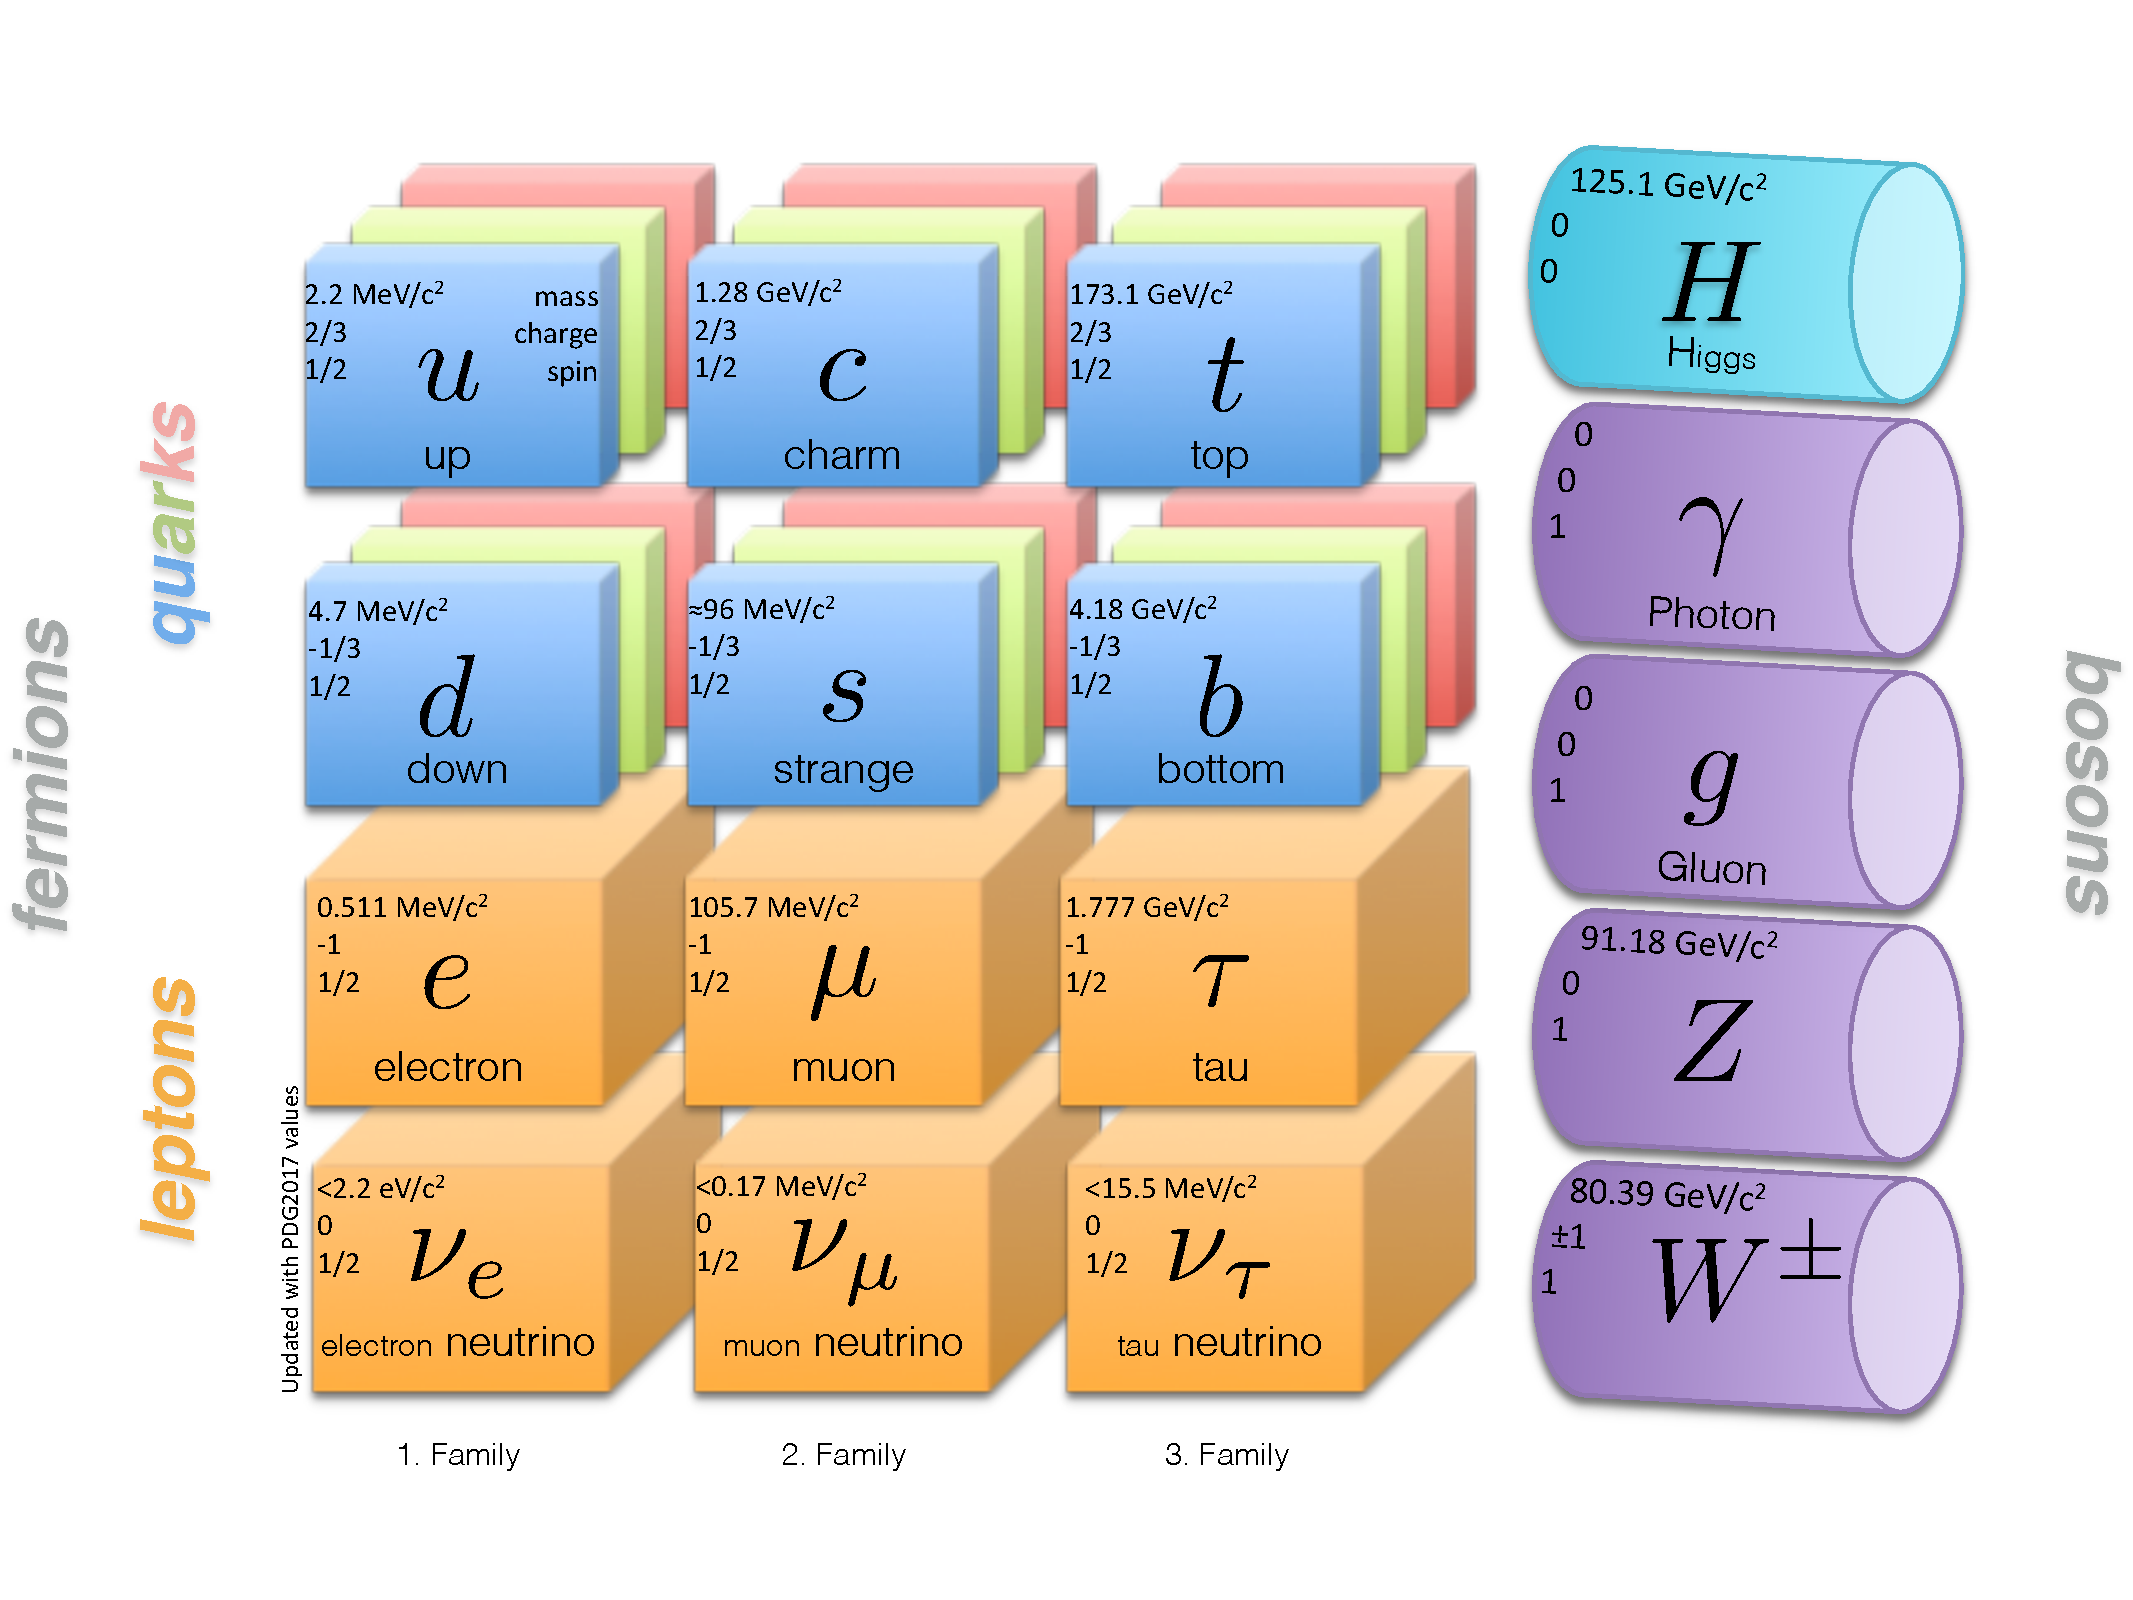
\includegraphics[width=0.8\textwidth]{Plots/SM/SM_eng}
  %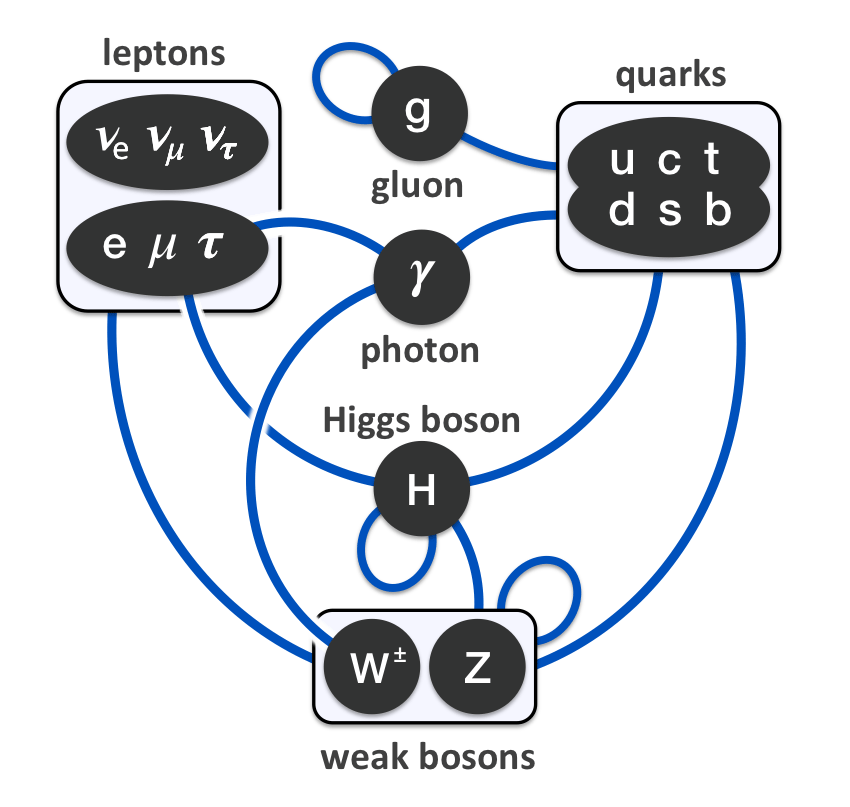
\includegraphics[width=0.35\textwidth]{Plots/SM/interactions}
  \caption{ All fundamental particles of the standard model, the gauge and Higgs bosons are shown in the diagram. The electric charge, spin and mass (or limit for neutrinos) are given in the corners of the boxes ~\cite{Olive:2016xmw}.
  %Righ: The ineractions of particles with each others and with themselves are shown in the diagram.
  }
  \label{fig:SM_particles}
\end{figure*}
The range of these forces is inversely proportional to their masses. The photon is massless so the range of electromagnetism is infinite while the range of weak force is constrained by the large mass of the corresponding gauge bosons. This mechanism is more complicated in the case of the strong force; it will be discussed in the next paragraphs.

\subsection{Standard Model: Particle Interactions}
\label{sec:StandardModelParticleInteractions}

The theory that aims to model strong force is called \textbf{quantum chromodynamics} (QCD). In Greek, the word $\chi\rho\hat{\omega}\mu\alpha$ chroma means color. 

After observation of bound states such as $\Delta^{++}_{(uuu)}$, violating Pauli\textquoteright s exclusion principle, it is suggested that the quarks possess three color (red , blue, green) charges. The interaction between quarks occurs through gluons. The fact that gluons have color charge make them interact with themselves as well. Accordingly, QCD also admits bound states whose valence constituents are all gluons, the non\-abelian gauge bosons of QCD. These additional mesons are one of the most important predictions of the SM and they are known as gluonia or glueballs. However, so far they have not been observed experimentally. For further reading, ~\cite{glueball1, glueball2} can be consulted.\\
QCD has two important postulates.
%an additional SU(3) gauge degree of freedom, 

Confinement:
In nature we observe only color singlet (colorless) particles. The particles with color charges, i.e. quarks and gluons, immediately coalesce to form colorless bound states (hadrons) given an attempt to separate them. This is also known as hadronization. As a result of this phenomenon, despite the fact that gluons are massless, the range of the strong force is confined. Moreover, in experiments a shower of color-neutral particles, which is called as jet and will be explained in Sec.\ref{sec:PFJET}, is observed instead of a single quark.

Asymptotic freedom:
The interaction of quarks becomes asymptotically weaker as the energy increases or as the distance decreases. In other words, the strong coupling constant $\alpha_s$  increases with distance, but inside a meson or a baryon, they act as free particles. This asymptotic freedom helps to build a perturbative description of QCD interactions; otherwise QCD calculations are extremely complicated.

%%%%
The interaction of charged particles with energies of the order of the $W^{\pm}$ boson mass can be described  by \textbf{quantum electrodynamics} (QED). The symmetry group of the electromagnetic theory is a unitary transformation $U(1)_{EM}$ and there is a massless field associated to the photon.
The $\beta$-decay, where the neutron decays to a proton, electron and corresponding antineutrino through the $W$ boson was explained by Enrico Fermi by an effective theory ~\cite{Fermi}. The theory is based on an $SU(2)_L$ symmetry group. The subscript “L” stands for the left handed particles. Due to lack of right handed neutrinos in nature, only left handed fermions contribute to the \textbf{weak interaction}.
In 1960s, Glashow-Salam-Weinberg proposed a unified theory of the QED and weak interactions ~\cite{glashow,salam,weinberg}.
After unification of the electric and the magnetic interactions by Maxwell, the unification of electromagnetic and weak interactions is an encouraging step towards the grand unified theories (GUT) that attempt to unify all interactions into a single theory. 
However, in the formulation of the SM, initially all the mass of particles are 0, in contrast to experiment.
Brout, Englert ~\cite{higgs1} and Higgs ~\cite{higgs2} solved the problem by implementing the electroweak symmetry breaking (EWSB), called BEH mechanism or only the Higgs mechanism. It introduces an additonal scalar field, the Higgs field. The SM Higgs boson is a Goldstone boson with mass given by $m_H=\sqrt{2\lambda}\nu$\footnote{$\nu=(\sqrt{2}G_F)^{-\frac{1}{2}}\approx$246GeV, $G_F$ is Fermi Coupling}. The massive bosons of weak interaction gain their mass through a non-zero vacuum expectation value (VEV) while for fermions direct Yukawa couplings to the Higgs boson provides their mass term.
Particles interact with the Higgs field at a different strength. Depending on the coupling between the Higgs field and the particle, its mass can be large or small. The Photons, having zero rest mass, do not couple to Higgs field. In the absence of the Higgs field, all the particles would be massless. 

%The SM particle content and their interactions were briefly covered in this section. 
%The chapter will continue with formulation of the SM.

\subsection{Standard Model: from the quantum field theory window }
\label{sec:StandardModelQFT}
In particle mechanics, a Lagrangian\footnote{L=T-V, T is the kinetic energy of the particle in a potential V.} is a function of the coordinates, and their time derivatives. In field theory a Lagrangian density is used and it is a function of the fields, $\phi_i$ and their position and time derivatives, $\partial_{\mu}\phi_i $. In relativistic theory, space and time coordinates are treated on equal footing. The Lagrangian plays an important role in physics because it encodes both the dynamics and the symmetries of the theory. Given a Lagrangian, the equation of motion from the Euler-Lagrange equations can be derived by considering the least action principle, i.e requiring that the variation of action is zero\footnote{$\delta S=0$, where $S=\int L dt$.}. Then, the Euler-Lagrange equation can be written as:
\begin{eqnarray}
\label{EuLag}
% \nonumber to remove numbering (before each equation)
	{ \partial_{\mu}\frac{\partial L}{\partial(\partial_{\mu}\phi_i)}} = {\frac{\partial L}{\partial\phi_i}} .
	%\,\frac{\patial}{\partial(\partial_{\mu}\phi_i)}
\end{eqnarray}
The SM is a relativistic quantum field theory (QFT).  Its Lagrangian is built on a global Poincar\'{e} symmetry, which implies symmetry under translations, rotations and Lorentz boosts. According to Noether\textquoteright s theorem ~\cite{Noether}, each continuous symmetry is accompanied by a conservation law. The Poincar\'{e}‬ symmetry implies the conservation to conservation of energy, momentum, and angular momentum. The gauge group of the SM, which is a local symmetry, is described as:  
\begin{eqnarray}
\label{SMsym}
% \nonumber to remove numbering (before each equation)
	{SU(3)_C \otimes SU(2)_L \otimes U(1)_Y}
\end{eqnarray}
where $SU(3)_C$,$SU(2)_L$ and $U(1)_Y$ are representing the gauge groups of the strong, weak and electromagnetic forces respectively. The subscript $C$ refers color, $L$ refers to left-handedness, and $Y$ refers hypercharge. 
The conserved quantities, which correspond to the symmetry in the Equation \ref{SMsym}, are color charge, charge, and weak hypercharge.\\
The rank of the group, i.e. the number of generators of the fields is at the same time the number of mediators, gauge bosons, of the corresponding vector field.
For instance, the $SU(3)_C$ group has eight\footnote{$N_c^2-1$, where $N_c=3$} generators thus it has eight vector fields which are called the gluon fields ($G_{\mu}$). Following the same argument, the $SU(2)_L$  group has three vector fields, ($W_{\mu}^1$, $ W_{\mu}^2$, and $ W_{\mu}^3$) and the $U(1)_Y$ group has only one vector field, ($B_{\mu}$). \\
In addition, the EWSB, or in other words the Higgs mechanism, leads to an additional scalar field, which will be denoted as $\phi$ in upcoming equations. 
The SM Lagrangian resides two components: $L_{QCD}$ and $L_{EWK}$. The first one is for strong interaction while the latter explains electroweak interaction including interaction with the Higgs boson. 
%\newpage
\begin{itemize}
  \item \textbf{Strong interaction}
\end{itemize}
As mentioned in the previous section, the theory that aims to model strong force is QCD. The QCD Lagrangian is given by:
\begin{eqnarray}
\label{LagQCD}
{L_{QCD}} = {\bar{\Psi}(i\gamma^{\mu}\partial_{\mu}-m)\Psi + g_s\bar{\Psi}T_aG_{\mu}^a\gamma^{\mu}\Psi - \frac{1}{4}G_{\mu\nu}^aG^{\mu\nu}_a}.
\end{eqnarray}
where $\Psi$ are the quark fields, $\gamma^{\mu}$ are the Dirac matrices, $g_s$ is the strong coupling constant, $T_a$ are Gell-Mann matrices and $G_{\mu\nu}^a \equiv \partial_{\mu}G_{\nu}^a - \partial_{\nu}G_{\mu}^a + g_sf_{abc}G_{\mu}^bG_{\nu}^c$\footnote{$f_{abc}$ are the structure constants}.
When constructing the Lagrangian, a covariant derivative is introduced such that the kinetic term stays invariant under gauge transformations. In general, the form of the covariant derivative is $D_{\mu}=\partial_{\mu}-igX_{\mu}$ where with the $g$ coefficient fermion interacts with the X boson. Concretely, the kinetic terms are read as $\bar{\Psi}\gamma^{\mu}D_{\mu}\Psi$, and the covariant derivative for QCD is defined as: $D_{\mu}=\partial_{\mu}-ig_sT_aG_{\mu}^a$.
%\newpage
\begin{itemize}
  \item \textbf{Electroweak interaction}
\end{itemize}

The electroweak Lagrangian, $L_{EWK}$, can be written as a sum of four contributions:
\begin{eqnarray}
\label{LagEWK1}
{L_{EWK} = L_{Gauge}+L_{Fermion}+L_{Higgs}+L_{Yukawa}}.
\end{eqnarray}
The covariant derivative that leaves this Lagrangian invariant under gauge transformations is described as: $D_{\mu}=\partial_{\mu}-igW_{\mu}^a\tau_a - ig'B_{\mu}Y_W$ where $g$ and $g'$ are the the gauge couplings of the $S U(2)_L$ and $U(1)_Y$ respectively. The $\tau_a$ denote the Pauli matrices. The weak hypercharge is denoted by $Y_W$ and it is defined as $2(Q-I_3)$. The electric charge is denoted by $Q$ and $I_3$ is the third component of the weak isospin.

The first term in Equation \ref{LagEWK1} is defining the interaction among the gauge bosons, and it can be written as:
\begin{eqnarray}
\label{Laggauge1}
{L_{Gauge} = -\frac{1}{4}W_{\mu\nu}^aW^{\mu\nu}_a -\frac{1}{4}B_{\mu\nu}B^{\mu\nu} }
\end{eqnarray}
where $W_{\mu\nu}^a = \partial_{\mu}W_{\nu}^a - \partial_{\nu}W_{\mu}^a + g\epsilon^{abc}W_{\mu}^bW_{\nu}^c$,
 $B_{\mu\nu} = \partial_{\mu}B_{\nu} - \partial_{\nu}B_{\mu}$.

The second term in Equation \ref{LagEWK1} stands for the fermion kinetic term and fermion interactions with $SU(2)$ and $U(1)$ bosons:
\begin{eqnarray}
\label{Lagfermions1}
{L_{Fermion} = i\bar{\Psi}\gamma^{\mu}D_{\mu}\Psi}
\end{eqnarray}

The third term in the same equation is the Higgs Lagrangian, describing the Higgs field, its self-interaction and its interaction with the gauge bosons:
\begin{eqnarray}
\label{LagHiggs1}
{L_{Higgs} = |D_{\mu}\phi|^2 - \lambda(|\phi|^2 - \frac{\nu^2}{2})^2},
\end{eqnarray}
where $\lambda$ is the Higgs self-coupling strength. %, $\nu$ is the vacuum expectation value (VEV) and $\nu^2 > 0$.
According to BEH mechanism, there is a scalar potential, which permeates the whole universe: 
\begin{eqnarray}
\label{higgspot}
% \nonumber to remove numbering (before each equation)
	{V(\Phi)}= {m^2\Phi^{\dagger}\Phi+\lambda(\Phi^{\dagger}\Phi)^2},
\end{eqnarray}
with the Higgs field $\Phi$ with weak hypercharge $Y =1$, and a self-interacting SU(2) complex doublet in Equation \ref{higgsfield}\footnote{$\phi^0$:CP-even,$a^0$:CP-odd neutral component. $\phi^+$:complex charged component}.
\begin{eqnarray}
\label{higgsfield}
% \nonumber to remove numbering (before each equation)
	{\Phi}= {\frac{1}{\sqrt2}}{\sqrt2\phi^{+}  \choose \phi^0 + ia^0 }
\end{eqnarray}

If the quadratic term is negative, the neutral element of the scalar doublet gains a non-zero vacuum expectation value (VEV) stimulating the spontaneous breaking of the SM gauge symmetry (SSB) \cite{Olive:2016xmw}.

The final term in equation \ref{LagEWK1}  is the Lagrangian of the Yukawa interaction between the Higgs field and the fermion fields (quarks and leptons). The $L_{Yukawa}$ produces fermion masses through spontaneous symmetry breaking. It can be written in the most general way ~\cite{srednicki}:
\begin{eqnarray}
\label{LagYukawa1}
{L_{Yukawa} = -\epsilon^{ij}\phi_i\ell_{jI}y_{Ij}\bar{e}_j - \epsilon^{ij}\phi_iq_{\alpha jI}y'_{Ij}\bar{d}_{j}^\alpha - \phi^{\dagger i}q_{\alpha iI}y''_{Ij}\bar{u}_{j}^\alpha +h.c.}\,
\end{eqnarray}
where $y_{Ij}$, $y'_{Ij}$, $y''_{Ij}$ are complex $3\,\times\,3$ matrices, and the generation indices ($I=1,2,3$) are summed.
After SSB the neutral and charged current interactions between fermions and gauge bosons can be derived from the $L_{EWK}$.  In order to extract the actual mass terms, a switch between basis with $W^a$, $B$ fields and a basis with mass eigenstates is desirable:
\begin{eqnarray}
\label{Zbos}
% \nonumber to remove numbering (before each equation)
	{ \gamma \choose Z } = { cos \theta_W \, \,\, \, sin \theta_W \choose -sin \theta_W \,\, cos \theta_W  } { B^0 \choose W^3 }
\end{eqnarray}
\begin{eqnarray}
\label{Wbos}
% \nonumber to remove numbering (before each equation)
	{W^{\pm}}= {W^1+iW^2} .
\end{eqnarray}
The $\theta_W $ term is the Weak mixing angle or Weinberg angle. This quantity is measured experimentally as well.

A more comprehensive and pedagogical formulation of the SM can be found in ~\cite{srednicki,Olive:2016xmw}. The next section will continue with experimental status of the SM.

%\newpage


\subsection{Standard Model: Experimental results}
\label{sec:StandardModelExp}

The entire SM particle content was discovered up to now. The fermionic substance was completed with the discovery of the top quark by the CDF and D$\O$ experiments in 1995 ~\cite{top1,top2}. In 2012, a particle, with a mass of approximately 125 GeV, which has similar features to the Higgs boson predicted by SM was discovered by ATLAS and CMS experiments ~\cite{higgsexp1,higgsexp2}.  Further studies with a much larger data set have provided precise measurements on its mass, production and decay rates. Results present consistency with the SM prediction, within errors. 
 With this new discovery, the bosonic content of the SM is also completed.\\
Testing the SM is not limited to collider experiments. In fact due to the technological constraints, probing the energies much larger than TeV scale is not possible with collider experiments; this much high energy can only be studied by cosmological experiments. In addition to cosmological and collider experiments, there are smaller scale desktop experiments where particle properties can be further investigated with high precision in lower energies ($\leq$GeV).
In the Figure \ref{tab:SM_tests}, an overview of the different types of experiments probing the SM can be seen. In addition to this, an example list of different kinds of measurements is also added to the table. The colors are making an analogy to the degree of the consistency of the measurements with the SM where green indicates that the experimental results are consistent with SM, yellow is showing that the measurements point out a deviation from SM predictions, and red evince that there must be a theory beyond the SM. Taking into account that not all the colors are green, the SM has several shortcomings not only from the experimental but also from theoretical perspective.  These shortcomings are the topic of the next section.
%\newpage
\begin{figure*}[!hb]
\centering
  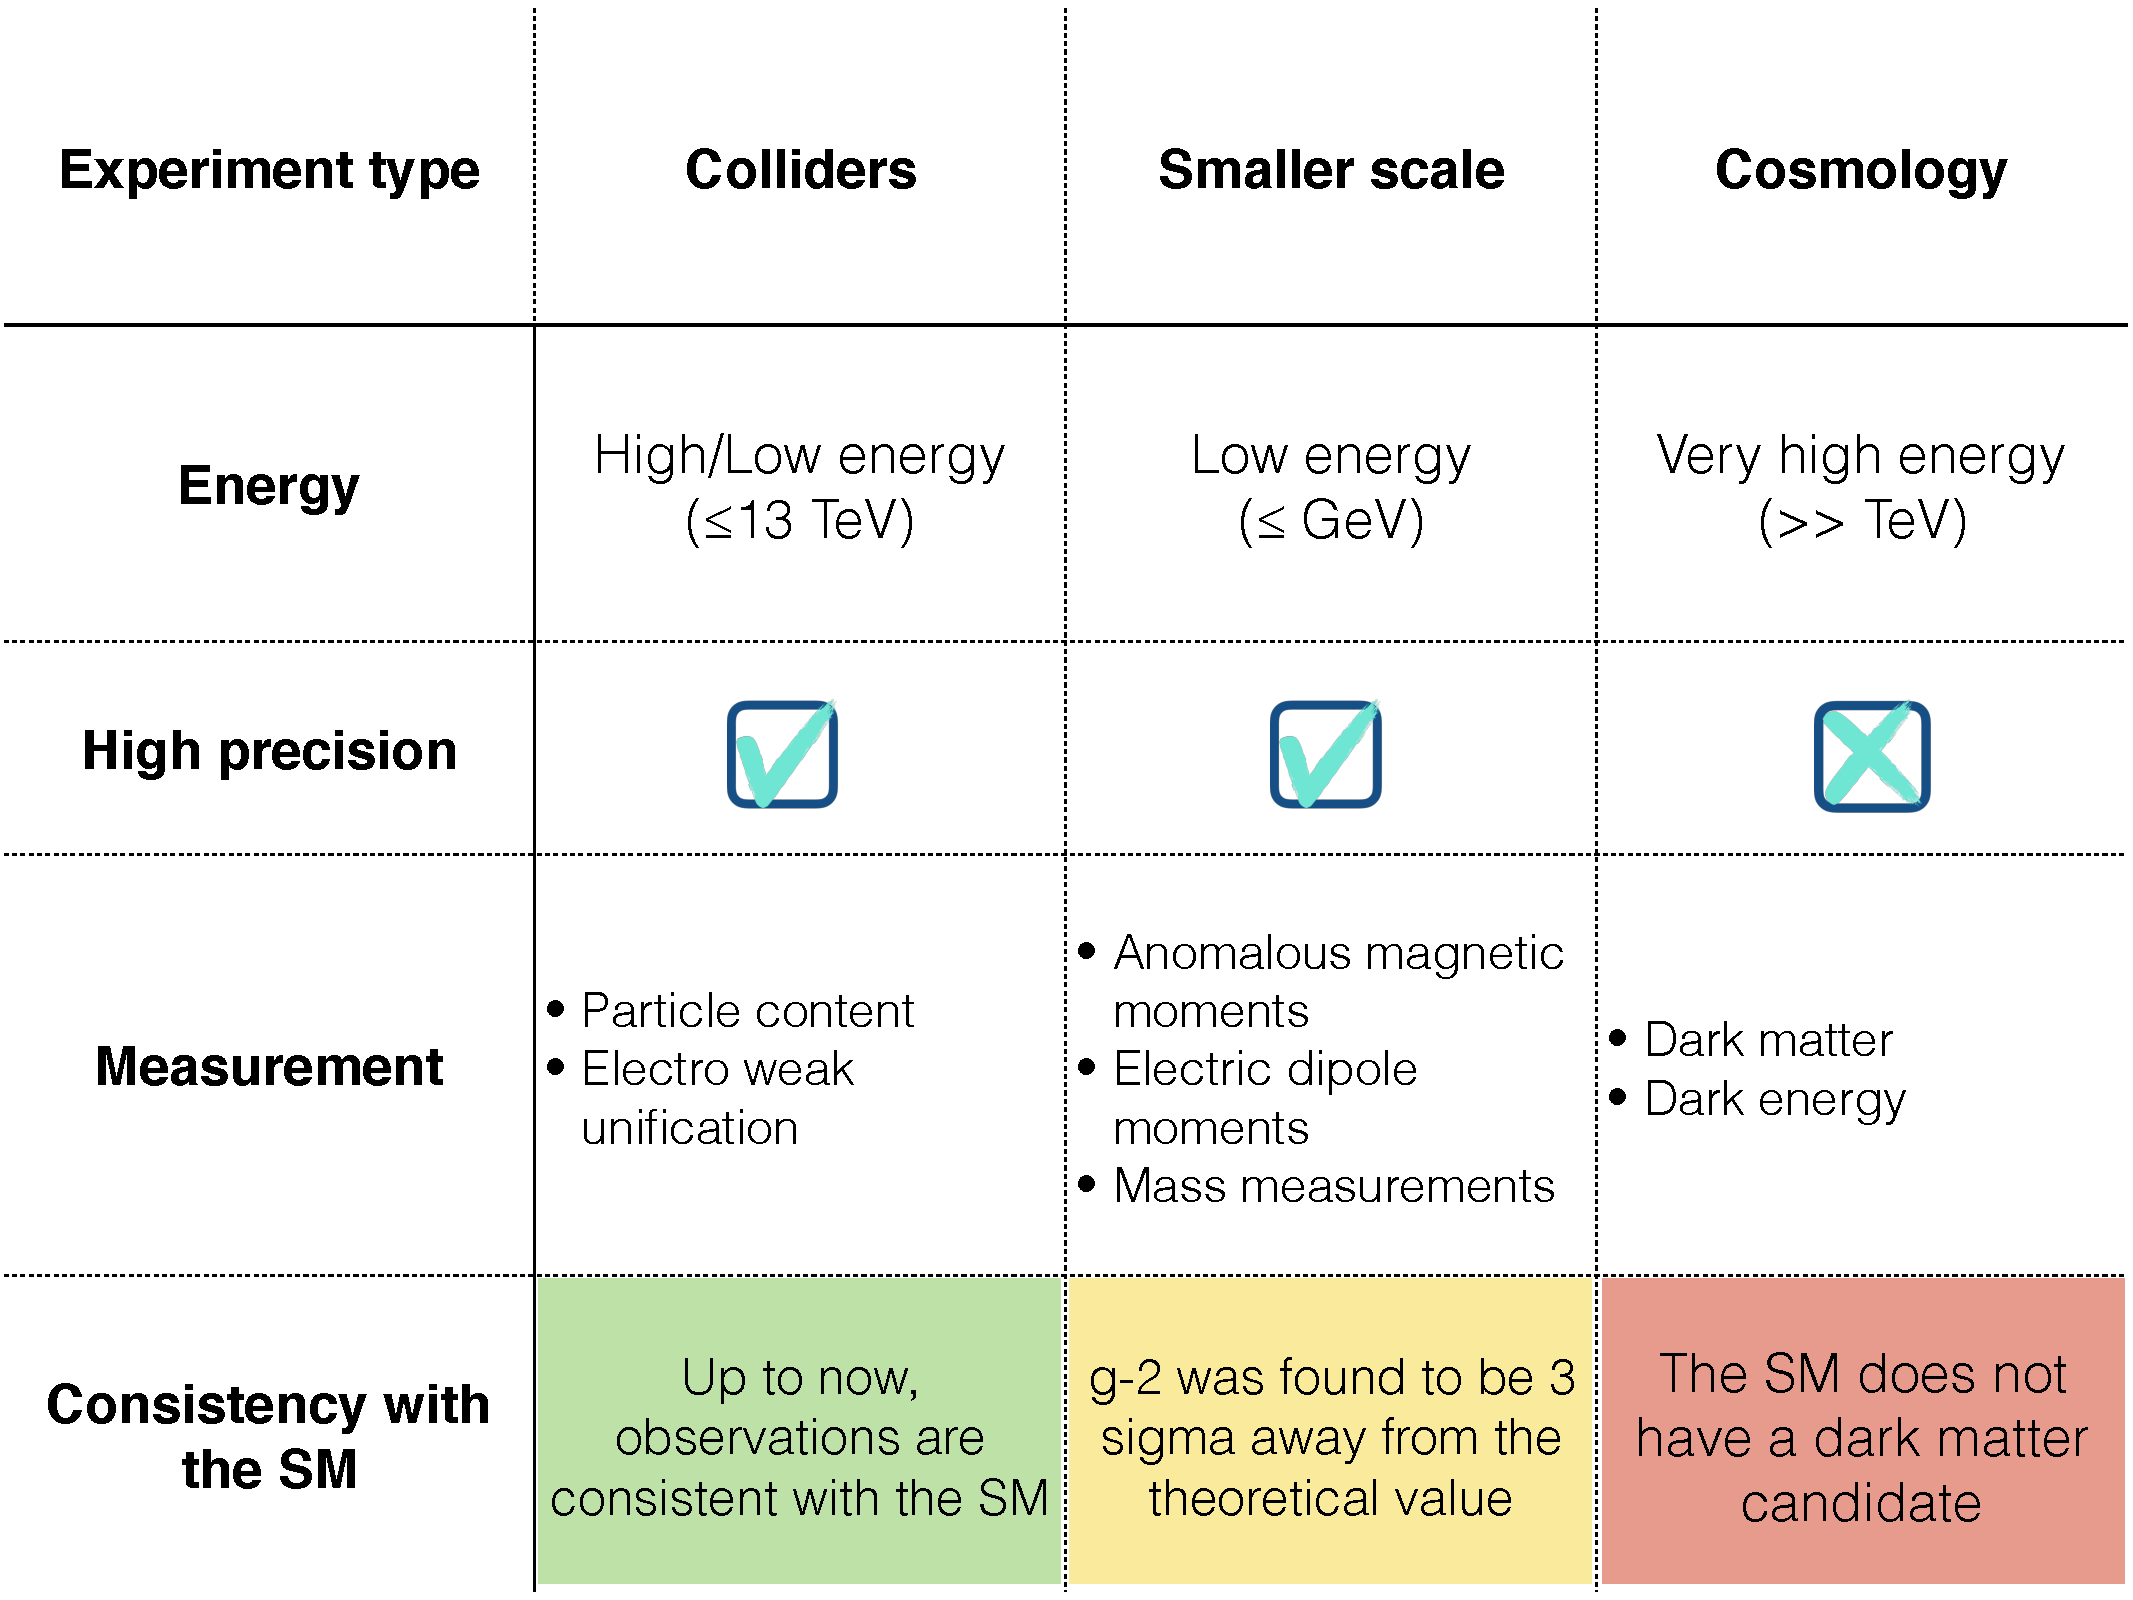
\includegraphics[width=0.8\textwidth]{Plots/SM/experiments.pdf}
  \caption{ An overview of characteristics of the experimental tests of the SM is shown in the table. 
  The information is mainly collected from ``the Electroweak model and constraints on new physics'' section in PDG2017 ~\cite{Olive:2016xmw} . Additionally further information on g-2 measurements can be found from the paper published by Muon G-2 experiment ~\cite{g2}.}
  \label{tab:SM_tests}
\end{figure*}
%\newpage
\subsection{Shortcomings of the Standard Model}
\label{sec:shortcomingsOfSM}
As mentioned in the previous section, no evidence of the new physics beyond the SM has been found at LHC. Moreover, up to now, the SM has successfully explained the world of subatomic physics. So, why are we searching for what is beyond the SM?  
\begin{itemize}
  \item \textbf{Experimental reasons}
\end{itemize}

\textbf{Lacking explanation of Gravity:} Certainly, the observation of gravitational waves is one of the two most exciting discoveries of our century. The announcement was done by LIGO and Virgo collaborations on 11 Feb 2016 ~\cite{LigoVirgo}. The observed waveform satisfies the predictions of general relativity ~\cite{GR}.
However, unless the gravitational field is quantized, it is impossible for the SM to include gravity.

\textbf{No Dark Matter candidate:} In 1933, Zwicky observed an unseen mass by applying the Virial theorem\footnote{relates the gravitational potential energy of a system to its kinetic energy} to the Coma cluster. He introduced this unseen mass as Dark matter (DM), originally in German called \textit{dunkle Materie} \cite{DM1}. The evidence of the DM got stronger with the observations made by V. Rubin and K. Ford on the velocity curve of more than twenty spiral galaxies ~\cite{DM2}.  Moreover, the observations of anisotropies in the cosmic microwave background (CMB) further supported the existence of DM. The data provided by Planck experiment, successor of COBE ~\cite{DM4} and WMAP ~\cite{DM3} experiments, is in good agreement with the $\Lambda$CDM (Lambda cold dark matter) model ~\cite{DM5}. This model postulates a dark energy dominated (68\%) flat universe, with 5\% baryonic matter and 27\% dark matter. Therefore, given the SM does not provide a viable cold dark matter candidate\footnote{In this context, Neutrinos are hot (relativistic) particles}, in fact the SM fails to explain 95\% of our universe.

\textbf{Massless neutrinos:} The observation of neutrino oscillations ~\cite{Nu1,Nu2} implies that at least two of the neutrinos should have non zero mass\footnote{The oscillation frequencies are proportional to the mass difference of the neutrino flavors. Therefore, only upper bounds can be measured.}. Neutrino masses can be included as an input to fermion Yukawa couplings, otherwise massless. However, even this input does not explain the observed mass differences between the generations. 

%\newpage
\begin{itemize}
  \item \textbf{Theoretical reasons}
\end{itemize}
Addition to the solid experimental reasons, the SM has also theoretical insufficiencies, which are mostly aesthetic concerns of theorists.

\textbf{Grand Unification:}
The unification of forces has started with the integration of electric and magnetic forces into one electromagnetic force. Then it was followed by the unification of electromagnetic and weak forces into the electroweak interaction. At this point, it is inevitable that one expects the merge of electroweak and strong interactions. In fact, the running couplings of electroweak and strong forces, as seen in the Figure \ref{fig:GUT}, meet at around 10$^{16}$ GeV. Finally, even the unification of gravity with other fundamental forces is strongly encouraged. 
\begin{figure*}[!hb]
\centering
  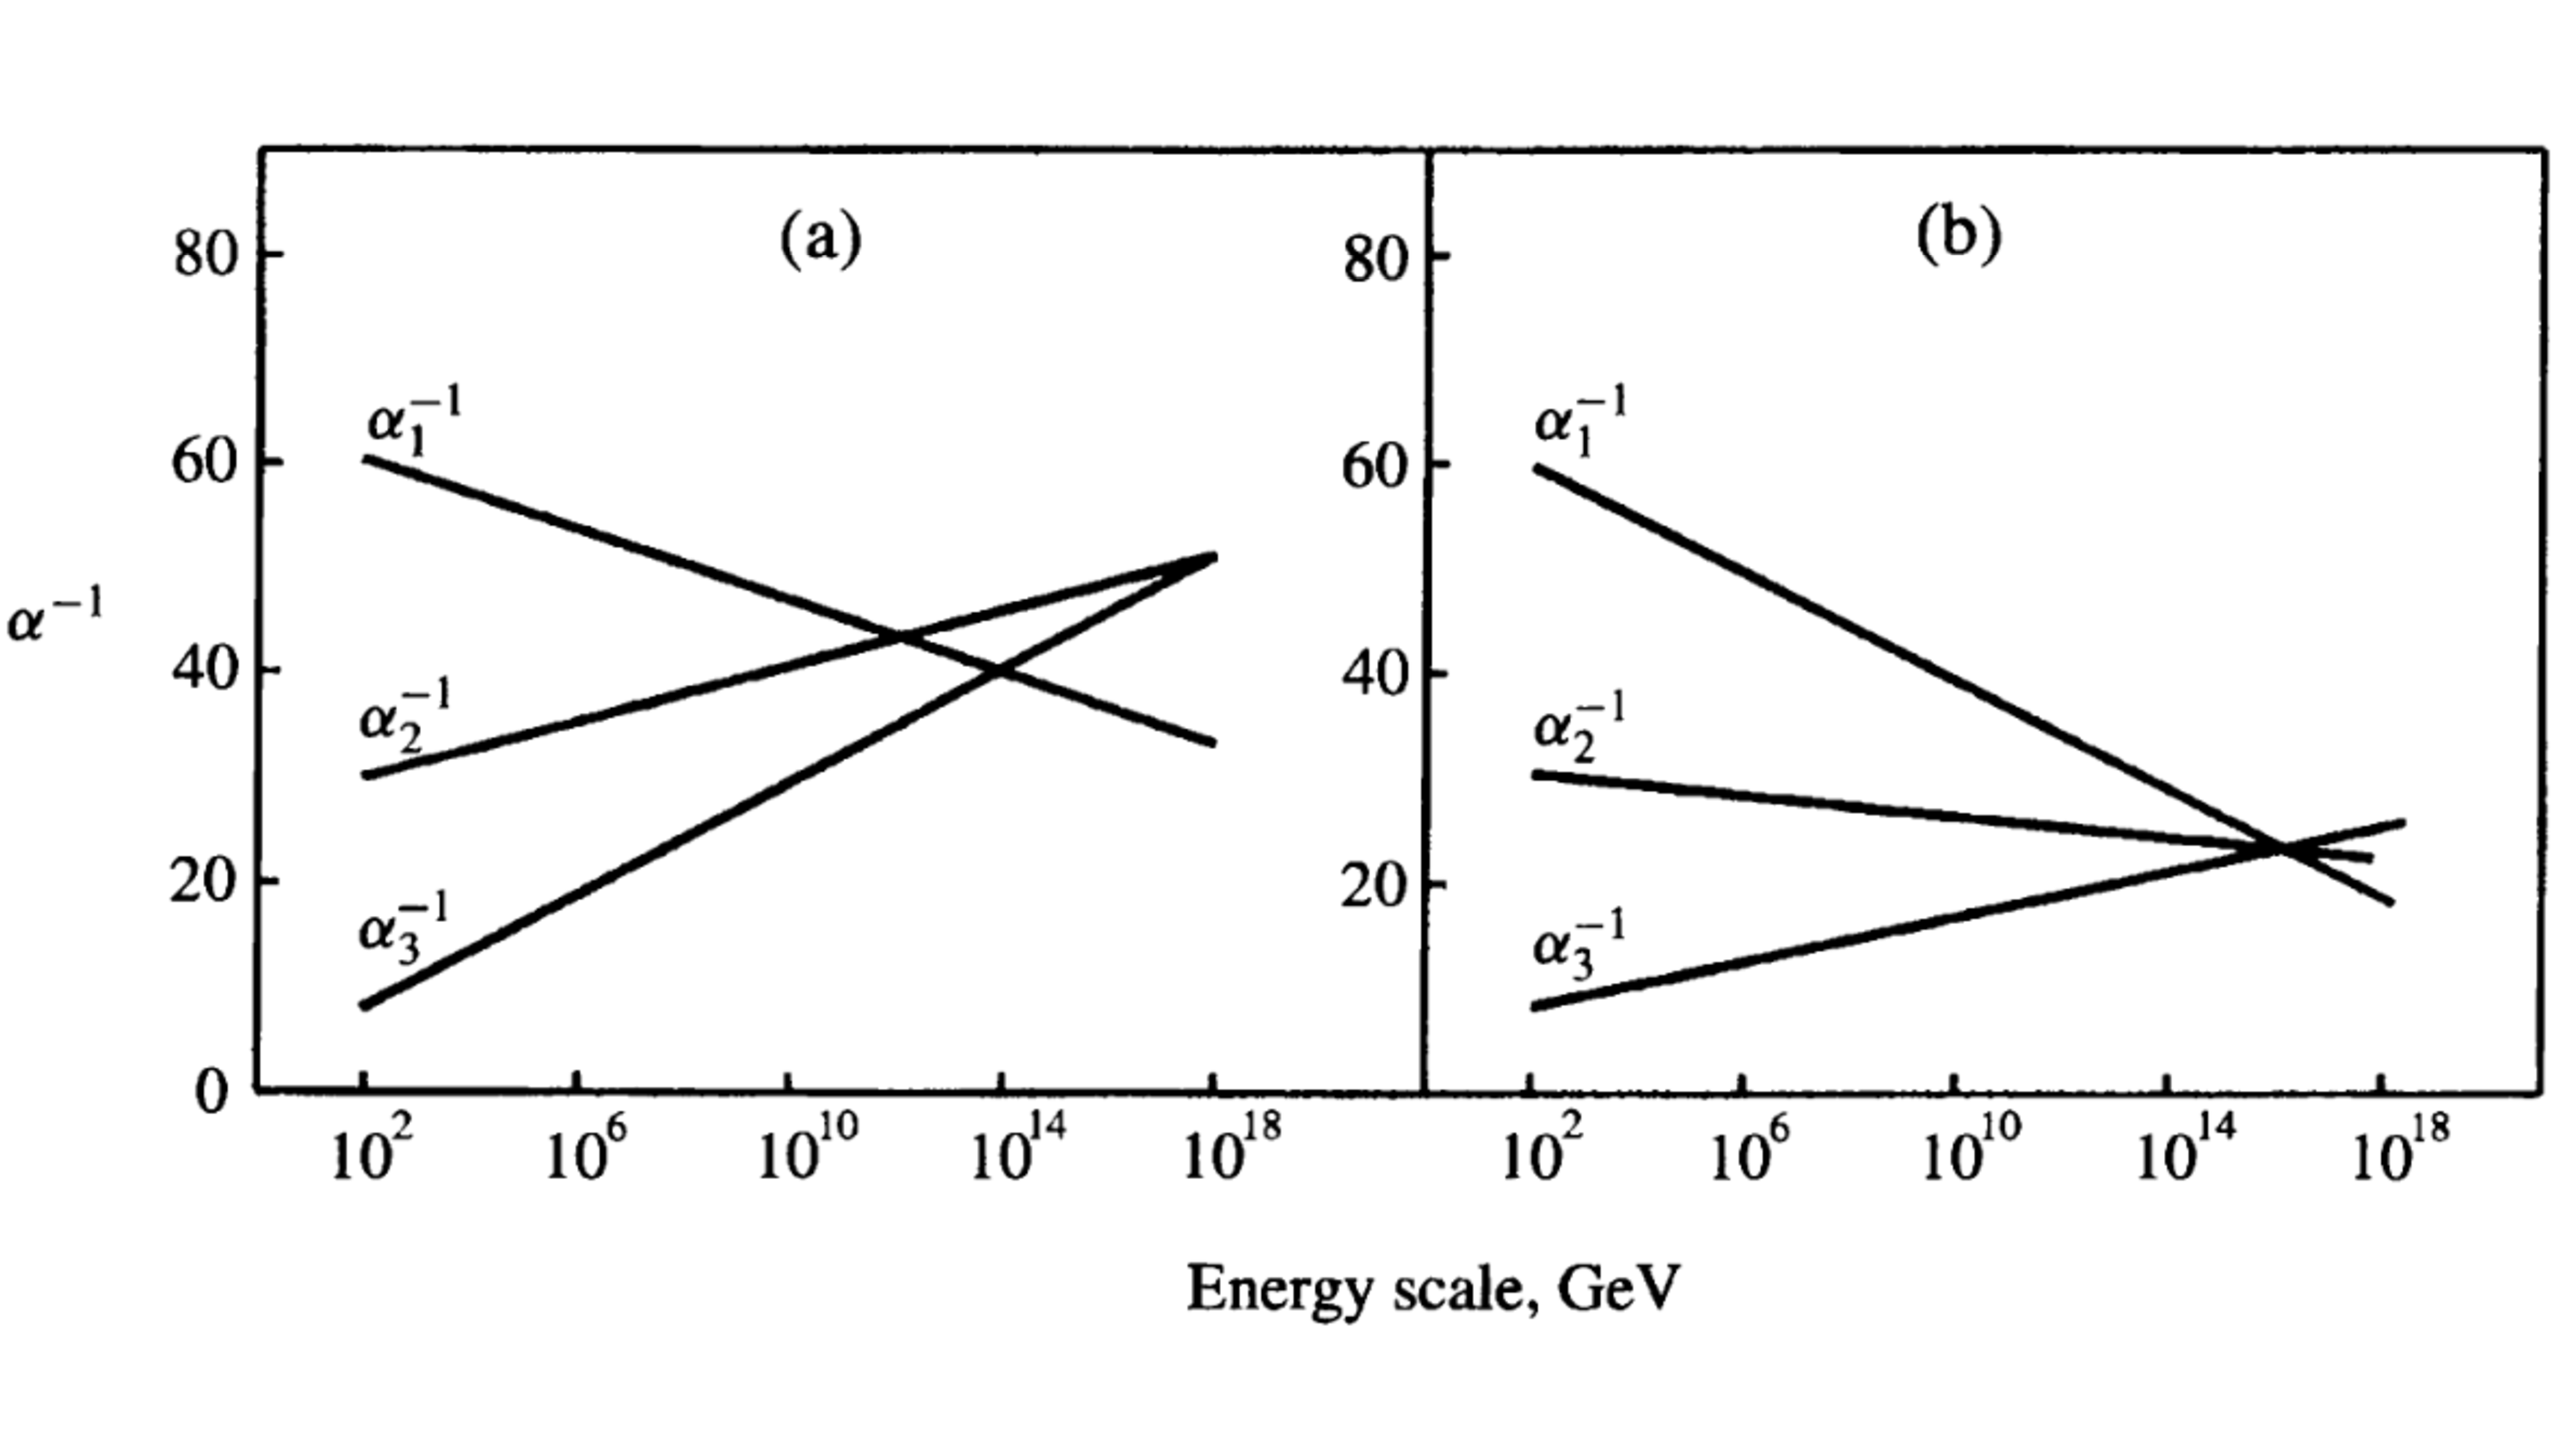
\includegraphics[width=0.8\textwidth]{Plots/BSM/GUTBoth.pdf}
  %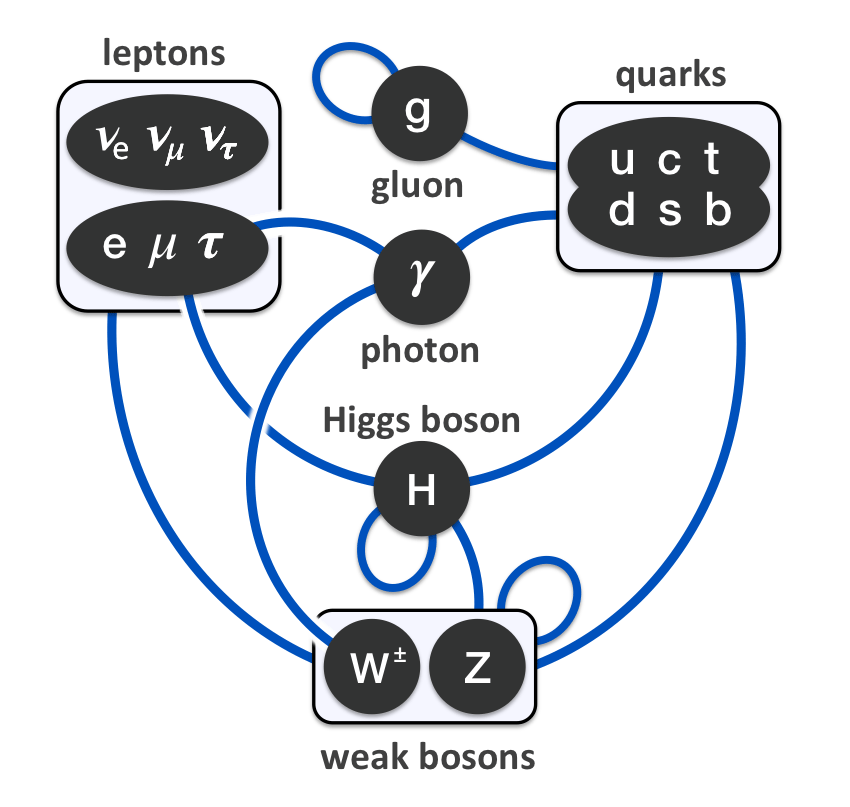
\includegraphics[width=0.35\textwidth]{Plots/SM/interactions}
  \caption{ The running couplings of U(1), SU(2), SU(3) is denoted by $\alpha_1$, $\alpha_2$, $\alpha_3$ respectively. The figure represents the evolution of inverse of couplings with energy scale, for (a) non-supersymmetric SU(5) and (b) supersymmetric SU(5). The figure is taken from ~\cite{perkins} pg. 282.
  }
  \label{fig:GUT}
\end{figure*}
\textbf{Hierarchy problem:}
In the literature of particle physics, there are two kinds of hierarchy problems; the big and the little hierarchy problem. The first one is due to the huge difference between mass scale of weak forces ($m_W$) and gravity (Planck scale\footnote{The Planck scale is the scale at which classical gravity theory is no longer valid but quantum gravity dominates. $M_P=2.4$x$10^{18}$GeV}).
In fact, this is not a consistency problem but a naturalness problem. The latter, the little hierarchy problem, is a problem of how large $m_{H}^2$, in Eq.\ref{higgspot}, can get. It receives huge quantum corrections because Higgs boson, including itself, couples to all massive particles in the SM. This subject will be discussed carefully in the upcoming sections.

There are many Beyond the Standard Model (BSM) theories claiming to solve some of the aforementioned SM shortcomings. The candidate BSM theory must not belie the current observations; on the contrary it should predict them. Moreover, in order to be able to test the theory, it should also provide a phenomenological background. 
In a spectrum of BSM theories which satisfies these constraints, the Supersymmetric extensions of the SM are the most promising ones.
This thesis focuses on a subgroup of these models, thus a relatively specified overview will be given in the following section. 
%%%%
%\newpage

\begin{figure*}[!hb]
\centering
  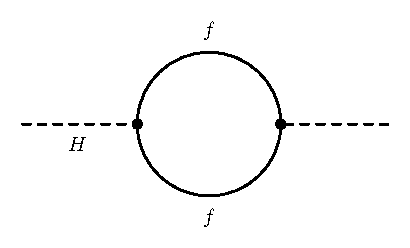
\includegraphics[width=0.3\textwidth]{Plots/feyndiagrams/susy_loop1.pdf}
    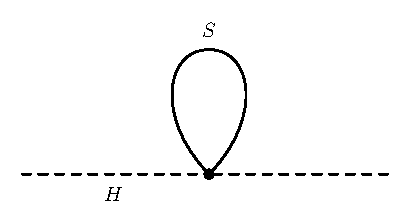
\includegraphics[width=0.3\textwidth]{Plots/feyndiagrams/susy_loop2.pdf}
  \caption{\label{fig:higgsloop} One-loop quantum corrections to the Higgs squared mass parameter $m_{H}^2$, due to (left) a Dirac fermion f, and (right) a scalar S ~\cite{SUSY1} p.g. 3}
\end{figure*}

%%%%%%%%%%%%%%%%%%%SUPERSYMMETRY%%%%%%%%%%%%%%%%%
%{\bf FIXME}
%{\bf The rest of the document has not been crosschecked yet.}
%{\bf FIXME}
\section{Supersymmetry as a solution}
\label{sec:susySol}
This chapter presents a brief summary of ~\cite{SUSY1} in the context of this thesis search.
When searching what is beyond the SM, a familiar concept, symmetry, helped again.  A symmetry, which relates fermionic states to bosonic states, had already attracted physicists' attention in the first half of the twentieth century. It was in the 1970s; a theory of four-dimensional relativistic space-time (super)symmetry has emerged. This theory is known as Supersymmetry (SUSY).  The supersymmetric transformation changes the spin angular momentum of the original SM fields by a factor of $\frac{1}{2}$ and this turns fermionic states into bosonic states, and vice versa.  These additional partners are called superpartners.  If these superpartners exist in TeV scale it can overcome several problems mentioned in section \ref{sec:shortcomingsOfSM}. \\
The existence of SUSY may lead to spectacular results that can be listed as follows:\\
\\
\textbf{Solving the hierarchy problem:}
\\
As mentioned in the previous section, Higgs boson couples to each massive SM fermion $f$ through a Yukawa coupling  $\lambda_f$. Therefore, the Higgs boson bare mass, the $m^2$ term in Equation \ref{higgspot}, receives enormous quantum corrections. The one-loop radiative correction terms (see Figure \ref{fig:higgsloop} left) which are coming from Dirac fermions $f$ are as follows:
\begin{eqnarray}
\label{deltaH1}
{\Delta m_H^2 = - \frac{|\lambda_f|^2}{8\pi^2}\Lambda_{UV}^2+...}
\end{eqnarray}
where $\Lambda_{UV}$ is an ultraviolet momentum cutoff, which is used to restrict the loop integral. The cutoff can be interpreted as the energy scale at which the new physics expected. 
Considering the top quark is the one with the largest mass among the SM fermions, the largest correction comes from it with $\lambda_f \approx 0.94$. If $\Lambda_{UV}$ is of the order the Planck mass, then this correction to $m_H^2$ is around 30 orders of magnitude larger than the Higgs bare mass.
In addition to the correction term given in Equation \ref{deltaH1}, a similar correction can be assumed from the heavy scalar particle $S$ (see Figure \ref{fig:higgsloop} right) as:
\begin{eqnarray}
\label{deltaH2}
{\Delta m_H^2 =  \frac{\lambda_S}{16\pi^2}\Lambda_{UV}^2+...}
\end{eqnarray}
where $\lambda_S$ is the coupling strength between the scalar particle and the Higgs field. 
It should be noted that this time correction carries an opposite sign. In this way, the diverging terms can be eliminated if a scalar particle exist with $\lambda_S = \frac{1}{2}|\lambda_f|^2$.\\
SUSY overcomes the hierarchy problem by introducing the so-called superpartners, which possess the same quantum numbers with original fields except for the spin.
As long as the masses of the superpartners are of the order O(TeV), SUSY can still be considered as natural. In order to achieve  this, the SUSY breaking needs to be soft. This means that it remains a valid symmetry of the underlying laws of physics but is broken in the course of the evolution of the state of the universe.
\\
\\
\textbf{Dark matter candidate:}
\\
The lower limit on the proton lifetime is set to $10^{30}$ years by experiments carried out in the water Cherenkov detector at Super Kamiokande in Japan ~\cite{protonLifetime}. This fact strongly suggests that the baryon number is conserved.  Unlike the SM, in SUSY theories the baryon and lepton number conservations can be violated. In SUSY, to prevent proton decay, a new quantum number, called as R-parity is introduced: 
\begin{eqnarray}
\label{Rparity}
{R =  (-1)^{3B+L+2S}}\,,
\end{eqnarray}
where $B$ represents the baryon number, $L$ is the lepton number, and $S$ denotes the spin.
All the SM particles have positive R-parity, while the superpartners have negative R-parity. Conservation of R-party entails that the SUSY particles can only be produced in pairs. Moreover, in SUSY, this conservation leads to a stable the lightest supersymmetric particle (LSP).  LSP is neutral in terms of both electric and color charge. Thus it is one of the most viable cold dark matter candidates and it has great importance in this thesis. If it exists, it would appear as a high missing energy in the events observed by experiments.
There are also R-party violating SUSY theories, but these are beyond the scope of this work. 
\\
\\
\textbf{Unification of gauge couplings:}
\\
Precise measurements of the running weak, strong and electromagnetic couplings performed at the Large Electron-Positron Collider (LEP) indicates that these couplings fail to unify at high energy (see Figure \ref{fig:GUT} a) ~\cite{ALEPH,GUTLep}. In ~\cite{GUTLep}, it is shown that the minimal supersymmetric standard model (MSSM) is the only possibility, without an intermediate mass scale. The MSSM can raise the scale of the unification by introducing a particle called the gluino, the spin half partner of the gluon. The gluino partially cancels the asymptotic freedom effect of the gluon itself ~\cite{Wil}.
The MSSM and its particle content will be explained in section \ref{sec:mssmPartContect}.
\\
\\
\textbf{Including gravity:}
\\
Even if it is not the subject of this thesis, it is worth mentioning that there is a SUSY model including gravity, namely supergravity. This model introduces a spin-2 massless gauge field, the graviton, which mediates gravity with its superpartner, the gravitino.  Supergravity, like any other QFT of gravity, is also not renormalizable.
\subsection{Algebra of Supersymmetry}
As it is stated in the beginning of this chapter, a SUSY transformation turns a bosonic state into a fermionic state, and vice versa. SM particles and their superpartners constitute supermultiplets.  For each of the chiral\footnote{left- and right- handed} SM fermions, there is a separate scalar partner and together they form chiral supermultiplets. The supersymmetric transformation operator $Q$ can also be called as supercharge operator, can be read as:
\begin{eqnarray}
\label{Q}
Q\ket{fermion} = \ket{boson} \\
Q\ket{boson} = \ket{fermion}.
\end{eqnarray}
In SUSY, the number of supercharges characterizes the theory. If there is only one supercharge then it is called a N=1 supersymmetry.  If there are two supercharges then there is a N=2 supersymmetry and so on. 
For chiral fermions, generators $Q$ and $Q^{\dagger}$ satisfy the commutation and anti-commutation relations:
\begin{eqnarray}
\label{Qrelations}
{\{Q,Q^{\dagger}\}=P^{\mu} \, , \, \{Q,Q\}=\{Q^{\dagger},Q^{\dagger}\}=0 \,,\, [P^{\mu},Q]=[P^{\mu},Q^{\dagger}]=0}
\end{eqnarray}
where $P^{\mu}=(H,\overrightarrow{p})$ stands for the spacetime momentum operator in which $H$ is the Hamiltonian and $\overrightarrow{p}$ is the three-momentum operator. 
Similar to chiral supermultiplets, the SM gauge bosons together with their fermionic supersymmetric partners form gauge supermultiplets.
The algebra in Equation \ref{Qrelations} indicates that the partner and the superpartner states have the same mass. However, no scalar superpartners have been found yet, although it would be expected to detect low mass partners, like selectron, experimentally long ago. This indicates that the supersymmetry has to be broken and the superpartners have much larger mass.
%\newpage
\subsection{Minimal Supersymmetric Standard Model}
\label{sec:mssmPartContect}
The minimal supersymmetric extension of the standard model (MSSM) is the only irreducible representation of the SUSY algebra (the aforementioned N=1 supersymmetry case). In other words, this is the model with the least number of additional particles and degrees of freedom. All other representations can be reduced to combinations of chiral and gauge supermultiplets. The MSSM chiral supermultiplets are shown in the Table \ref{tab:mssmChiral} while the gauge multiplets are listed in the Table \ref{tab:mssmGauge}. 
As in the table, all superpartners are represented by a version containing a tilde ($^ {\sim} $) of the original SM particle symbols. The scalar counterparts, are indicated by adding an ``s'' as initials to the SM fermion names  (e.g. selectron) while the fermionic gauge superpartners are represented by appending ``ino'' (e.g gluino). The subscripts $L$ and $R$ of the sleptons show only the helicity of their SM partners.
\renewcommand{\arraystretch}{1.5}
\begin{table}[ht]
\begin{center}
\begin{tabular}{|c|c|c|c|c|}\hline
\multicolumn{2}{ |c| }{Names}         & Spin 0                        & Spin $\frac{1}{2}$ & $SU(3)_C,\,SU(2)_L,\,U(1)_Y$ \\
\hline
\hline
squarks, quarks & Q & ($\tilde{u}_L$\,\,\,$\tilde{d}_L$) & ($u_L$\,\,\,$d_L$)      & ( {\bf 3} , {\bf 2} , $\frac{1}{6}$)\\
\multirow{2}{*}{(x3 families)} &$\bar{u}$ &$\tilde{u}^*_R$  & $u^{\dagger}_R$     & ( $\bf\bar{3}$ , {\bf 1} , -$\frac{2}{3}$)\\
                                             &$\bar{d}$ & $\tilde{d}^*_R$ & $d^{\dagger}_R$     & ( $\bf\bar{3}$ , {\bf 1} , $\frac{1}{3}$)\\
\hline
sleptons, leptons & L & ($\tilde{\nu}$\,\,\,$\tilde{e}_L$) & ($\nu$\,\,\,$e_L$)      & ( {\bf 1} , {\bf 2} , -$\frac{1}{2}$)\\
(x3 families)       & $\bar{e}$ &   $\tilde{e}^*_R$ & $e^{\dagger}_R$    & ( {\bf 1} , {\bf 1} , 1)\\
\hline
\multirow{2}{*}{Higgs, higgsinos} &$H_u$ & ($H^+_u$\,\,\,$H^0_u$) & ($\tilde{H}^+_u$\,\,\,$\tilde{H}^0_u$)      & ( {\bf 1} , {\bf 2} , +$\frac{1}{2}$)\\
&$H_d$ & ($H^0_d$\,\,\,$H^-_d$) & ($\tilde{H}^0_d$\,\,\,$\tilde{H}^-_d$)     & ( {\bf 1} , {\bf 2} , -$\frac{1}{2}$)\\
\hline
\end{tabular}
\end{center}
\caption{Chiral supermultiplets of the MSSM}\label{tab:mssmChiral}
\end{table}
\\
\begin{table}[ht]
\begin{center}
\begin{tabular}{|c|c|c|c|c|}\hline
Names    & Spin $\frac{1}{2}$    & Spin  1 & $SU(3)_C,\,SU(2)_L,\,U(1)_Y$ \\
\hline
\hline
gluino, gluon & $\tilde{g}$  &  $g$      & ( {\bf 8} , {\bf 1} , 0)\\
\hline
winos, W bosons & $\tilde{W}^{\pm}$\,\, $\tilde{W}^0$  & $ W^{\pm}$\,\, $W^0$      & ( {\bf 1} , {\bf 3} , 0) \\
\hline
bino, B boson &  $\tilde{B}^0$ &    $B^0$   & ( {\bf 1} , {\bf 1} , 0)\\
\hline
\end{tabular}
\end{center}
\caption{Gauge supermultiplets of the MSSM}\label{tab:mssmGauge}
\end{table}
\renewcommand{\arraystretch}{1}
In MSSM, there are two Higgs chiral supermultiplets. They are the cure of the gauge anomaly, in other words, they leave the action invariant under the supersymmetry transformation. Moreover, by the construction of SUSY, the Higgs doublet with hypercharge $Y=\frac{1}{2}$ is only able to give masses to the up-type quarks while the one with hypercharge $Y=-\frac{1}{2}$ gives masses to the down-type quarks and charged fermions. Therefore, the $SU(2)_L$ complex scalar fields with hypercharge $Y=\frac{1}{2}$ and $Y=-\frac{1}{2}$ can be denoted by $H_u$ and $H_d$ respectively. The half spin superpartners are called higgsinos and represented as $\tilde{H}_u$ and $\tilde{H}_d$.\\
The gluino is a half spin color octet supersymmetric partner of the gluon.  The superpartners of the electroweak gauge bosons are called winos and binos. The mixing of $\tilde{W}^0$ and $\tilde{B}^0$ are called zino ($\tilde{Z}^0$) and photino($\tilde{\gamma}$).\\
Due to the EWSB the higgsinos and electroweak gauginos mix with each other. The mixing between neutral higgsinos and the neutral gauginos results in four mass eigenstates called neutralinos and denoted by \ninoi ($i = 1, 2, 3, 4$). Whereas, the charged higgsinos and winos combine to form two mass eigenstates called charginos denoted by \chipmi ($i = 1, 2$).\\
As mentioned when discussing the hierarchy problem, the breaking of SUSY needs to be soft. In the MSSM, SUSY breaking is introduced by including a new component ($L^{MSSM}_{soft}$) to the Lagrangian. The Lagrangian, then, can be read as:
\begin{eqnarray}
\label{Lsusy}
{L = L^{MSSM}+L^{MSSM}_{soft}}.
\end{eqnarray}
The Yukawa and gauge interactions are contained in the first term, $L^{MSSM}$, while the $L^{MSSM}_{soft}$ is breaking the symmetry.  In order not to cause ultraviolet divergences, $L^{MSSM}_{soft}$ includes only the terms with positive mass dimension. In this way, the correction terms of the Higgs mass contain only logarithmic divergences:
\begin{eqnarray}
\label{deltaH3}
{\Delta m_H^2 = -m^2_{soft}[ \frac{\lambda}{16\pi^2}ln(\Lambda_{UV}/m_{soft})+...]}\, .
\end{eqnarray}
In order to satisfy the natural requirement, $| \Delta m_H^2| < m_H^2|_{measured}$, $m_{soft}$ needs to be of the order of TeV scale. This indicates that the new particles introduced by MSSM, if they exist, should be reachable at the LHC. \\
The $L^{MSSM}_{soft}$ adds 105 new parameters to 19 parameters coming from pure SM. These 105 additional parameters are categorized as follows: 48 CP-violating phases in the gaugino/higgsino and squark/slepton sectors, and 21 squark/slepton masses with 36 mixing angles to define their mass eigenstates.\\
The large number of parameters of the MSSM make the interpretation of the experimental results challenging, even almost impossible.  Therefore, using universality assumptions at the Grand Unified Theory (GUT) scale, the number of free parameters is reduced to five. This model, appropriately, is called as the constrained MSSM (cMSSM). Another approach would be to focus on a limited set of SUSY particle production and decay modes and allow other parameters to change freely. This effective theory approach is called simplified models spectra (SMS) ~\cite{SMS} and in this thesis, results are interpreted in the context of SMS. Before introducing the simplified models, it is beneficial to give an overview of the MSSM particle decays. To stay in the scope of this thesis, only the R-parity conserving scenarios will be discussed. In these models, the cascade decays of SUSY particles always end with an LSP. In this search, the lightest neutralino, $ \ninoone$, is the LSP. A deepened version of the topic is presented in chapter 9 of ~\cite{SUSY1}.
\\
\textbf{Neutralino and chargino} are mixtures of the higgsinos and gauginos that are the spin half partners of the Higgs and gauge bosons. A neutralino or chargino can decay into lepton+slepton or quark+squark pairs, given the condition that slepton and squark are light enough. A neutralino or chargino may also decay into a Higgs scalar or an electroweak gauge boson via lighter neutralino or chargino. 
Therefore, the possible two-body decay modes for neutralinos and charginos in the MSSM are:
\begin{eqnarray}
\label{ChiDecays}
\ninoi \rightarrow Z \ninoj, \, W \chipmj,\,  h^0\ninoj ,\,l\tilde{l},\,\nu\tilde{\nu} \, ,\\
\chipmi \rightarrow W \ninoj,\, Z \chipm ,\, h^0\chipm,\,l\tilde{\nu},\,\nu\tilde{l} \, .
\end{eqnarray}
\textbf{Gluino} decays via a squark exclusively, which can be either on- or off-shell. If the on-shell decays are allowed, then $\tilde{g} \rightarrow t\tilde{t}$ and $\tilde{g} \rightarrow b\tilde{b}$ are probably the dominating channels. Otherwise the squarks are off-shell and this favors the following decays: $\tilde{g} \rightarrow qq\ninoi$ and $\tilde{g} \rightarrow qq'\chipmi$.
\\

%\newpage
\subsection{Simplified Models}
\label{sec:simplifiedModels}
The simplified model spectra (SMS) involves only a part of the parameter space of MSSM.  This simplification leaves a few phenomenologically relevant parameters to understand the SUSY models; the cross section, branching ratios, and masses.  In this simplified framework, normally a limited number of decay channels are considered. In other words, the branching ratios are set to 100\% or a linear combination of such models is used for mixed decays.  In this way, results can also be reinterpreted within other (non-)SUSY theories.\\
\textbf{An example model ($\tilde{g} \rightarrow q\bar{q}\ninoone$):}
\\
In this simplified model, gluino decays to two light quarks and a neutralino. Generally, the neutralino is considered to be the stable lightest supersymmetric particle or LSP. Hence, It is a strong candidate of Dark Matter. In this model conserning direct decay, the paramters include the mass of the gluino and neutralino ($m_{\tilde{g}}$, $m_{\ninoone}$) and the production cross section of the gluino $\sigma(pp\rightarrow \tilde{g}\tilde{g}+X$). The case where gluino decays to two light quarks and an intermediate chargino, with the latter decaying to a gauge boson and a neutralino can be read as:
\begin{eqnarray}
\label{2step}
\tilde{g} \rightarrow q\bar{q}\chipmone \rightarrow q\bar{q}(W^{\pm} \ninoone) \\
\tilde{g} \rightarrow q\bar{q}\ninotwo \rightarrow q\bar{q}(Z^0 \ninoone) .
\end{eqnarray}
In this case, the mass of the intermediate particle (chargino \chipmone or a heavier neutralino \ninotwo) is also included in the parameters. In order to reduce the three-dimensional mass space, chargino mass is considered to be dependent to gluino and neutralino masses. The relation is given by: $m_{\chipmone} = m{\ninoone} + r(m_{\tilde{g}} - m_{\ninoone})$. The kinematics of the decay strongly related to the value of r. To further decrease the number of parameters, the branching ratio of these decays is set to 100\%. \\
In simplified models of gluino pair production, the case where each gluino decays as shown in the Equation \ref{2step} with a r=0.5, which indicates the mass of the chargino is at the midway, is called T5qqqqWW while the direct decay of gluino to top quark pair and  a neutralino is called as T1tttt\footnote{this naming is used within the CMS collabration}. The diagrams for T1tttt and T5qqqqWW can be seen in Figure \ref{fig:diagrams} left and right respectively. In this thesis, the T5qqqqWW model is used to interpret the results which is well motivated in the searches at LHC \cite{t51,t52}. \\
\begin{figure*}[!hb]
  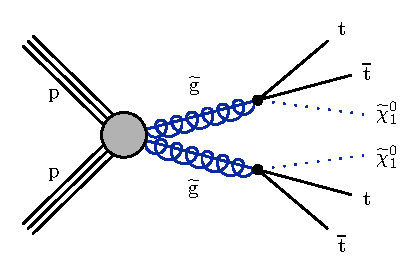
\includegraphics[width=0.35\textwidth]{Plots/feyndiagrams/T1tttt.pdf}
  \hfil
  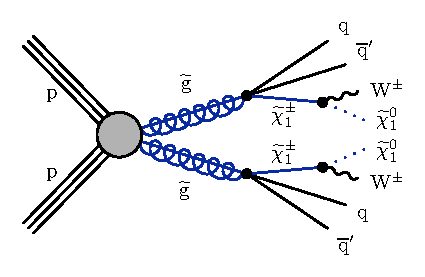
\includegraphics[width=0.35\textwidth]{Plots/feyndiagrams/T5qqqqWW.pdf}
  \hfil
\centering
  \caption{\label{fig:diagrams} Diagrams showing the simplified models T1tttt (left) and
T5qqqqWW (right).  %FIXME
%chargino ($\ensuremath{\widetilde{\chi}^{\pm}_1}$) and the neutralino ($\ensuremath{\widetilde{\chi}^0_1}$).
  }
\end{figure*}
\\
A variety of SMS approaches has been investigated by the ATLAS and CMS collaborations at the LHC. In the following, a short history of SUSY searches at colliders will be discussed.

%\newpage
\subsection{Short History of SUSY searches at colliders}
\label{sec:histSus}
%As an experimentalist to be able to decide where to look for new physics, it is essential to know what has been covered in the past. 
Before the LHC, the first constraints on SUSY had already been set by UA1 experiment and the UA2 experiment at Super Proton Synchrotron. It was until 2000, SUSY searches continued up to 209 GeV at the electron-positron collider LEP. Until 2011, The CDF and D$\O$ experiments at the Tevatron extended the limits in the context of cMSSM. In parallel between 1992 and 2007, the H1 and ZEUS experiments at HERA (The electron-proton collider) searched for the R-parity violating production of single SUSY particles. The LHC has started proton-proton collision at a center of mass energy of 7 TeV in 2010. Since then, ATLAS and CMS experiments have performed robust searches and provided strong limits in the context of SMS. The 2011 and 2012 runs of the LHC are called Run 1. During Run 1, 20 fb$^{-1}$ data was collected at a center of mass energy 7 and 8 TeV. In 2012, with the discovery of Higgs boson, the SUSY models have been constrained further. Later, in the first stage of Run 2, approximately 36 fb$^{-1}$ data has been collected at a center of mass energy 13 TeV. A summary of the both Run 1 and Run 2 results by ATLAS and CMS experiments is presented in Figure \ref{fig:susy_Summary} including the results from present search. Within the MSSM these results have already pushed the sparticle mass boundaries required to solve hierarchy/naturalness/fine-tunning problems. For instance, It was foreseen that the gluinos cannot be much heavier than 1 TeV and the higgsino mass should be around 200 GeV.  Obviously, the latest results challenge these requirements.  Nevertheless, there is still room for expanding the searches, for example, in the regions with compressed spectra where the analysis is not so trivial. 
\begin{figure*}[!hb]
\centering
  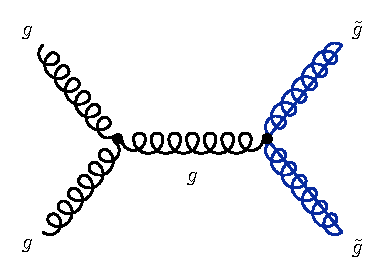
\includegraphics[width=0.18\textwidth]{Plots/feyndiagrams/gluinoprod_sch1.pdf}
   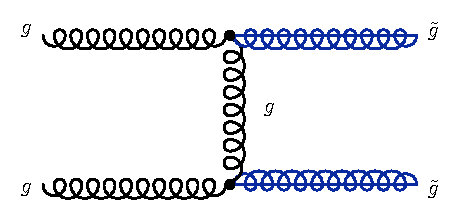
\includegraphics[width=0.25\textwidth]{Plots/feyndiagrams/gluinoprod_tch1.pdf}
   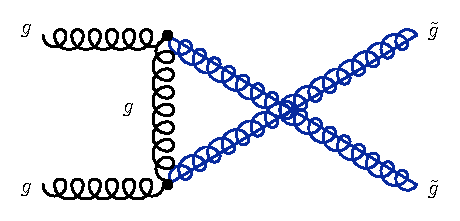
\includegraphics[width=0.25\textwidth]{Plots/feyndiagrams/gluinoprod_uch1.pdf}
  \\
    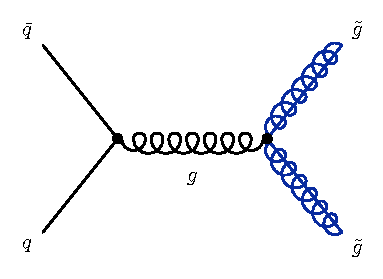
\includegraphics[width=0.18\textwidth]{Plots/feyndiagrams/gluinoprod_sch2.pdf}
   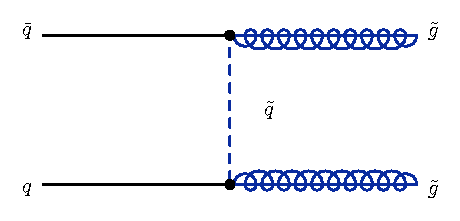
\includegraphics[width=0.25\textwidth]{Plots/feyndiagrams/gluinoprod_tch2.pdf}
    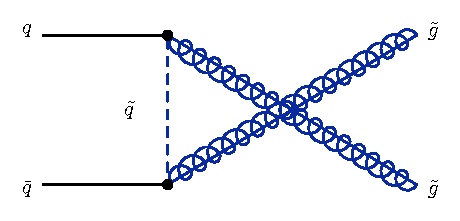
\includegraphics[width=0.25\textwidth]{Plots/feyndiagrams/gluinoprod_uch2.pdf}

  \caption{\label{fig:gluProd}Feynman  Diagrams showing the gluiono pair prodution.
  SUSY particles are  shown in blue.
  }
\end{figure*}
\begin{figure*}[!hb]
\centering
  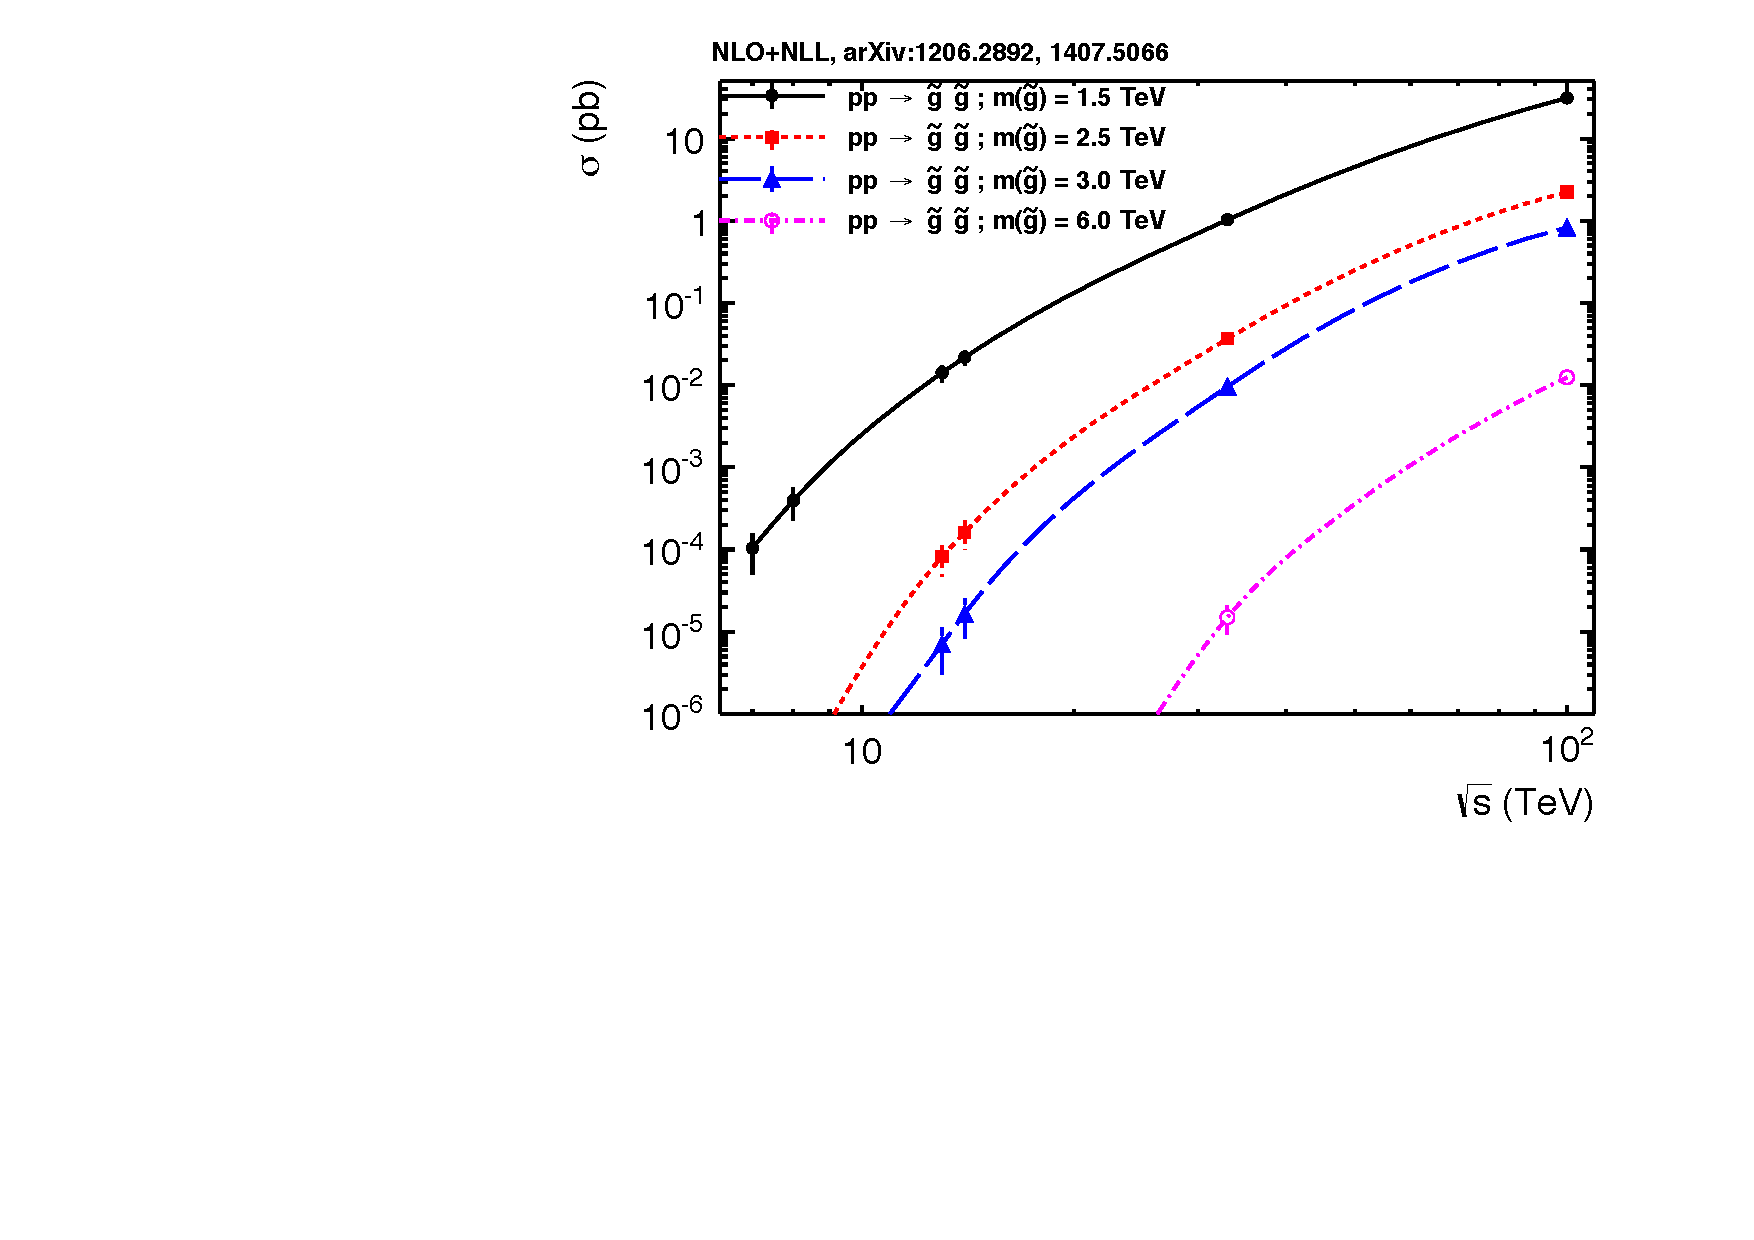
\includegraphics[width=0.4\textwidth]{Plots/SUSY/gluino_xsec}
  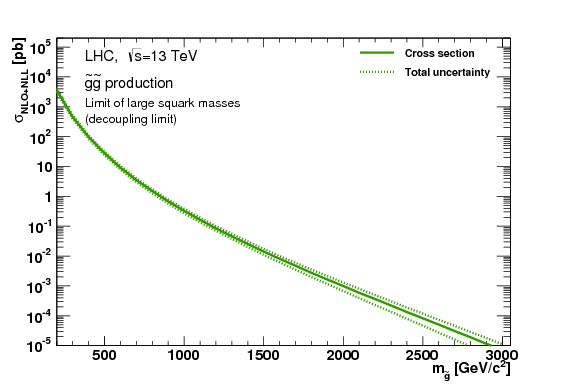
\includegraphics[width=0.42\textwidth]{Plots/SUSY/XSectionPlots_13TeV}
  \caption{ left: Cross sections of gluino pair production for four different mass points are given as a function of the center of mass energy. right: Cross section of gluino pair production at 13 TeV center of mass energy is given as a function of gluino mass.
  ~\cite{gluxsec}
  }
  \label{fig:glu_xsec}
\end{figure*}
%\newpage
\textbf{Expectations for gluino searches at 13 TeV:}
\\
LHC is a proton-proton collider. Consequently, high sensitivity is favored in the production of color charged particles: the gluino and squarks.\\
The gluino pair production diagrams are shown in Figure \ref{fig:gluProd}. The cross sections as a function of the center of mass energy and gluino mass are shown respectively in Figure  \ref{fig:glu_xsec} left and right. The cross section of gluino pair production increased significantly from 8 TeV to 13 TeV. However, the cross section of SM processes increased as well (see Figure \ref{fig:sm_xsec}). These figures indicate that at 13 TeV for 10$^{10}$ SM events, 1 event including gluino pair production is expected. This sounds even harder than looking for a 4-leaf clover. Nevertheless, it is still achievable by designing an analysis strategy, with a robust background estimation and assigning the uncertainties carefully. An example of such a search will be presented in this thesis and in the section \ref{sec:Comparison} a comparison of the latest results from gluino searches can be found.\\
%\newpage
\textbf{History of the present analysis:}
\\
As mentioned in the previous section, in the present thesis, a search for SUSY is performed in the context of the simplified model T5qqqqWW. The analysis journey started in Run1 with a search for a similar model, which was T1tttt. In this model, the presence of 2 top-antitop quark pairs requires a search for multiple b-tagged (see Sec. \ref{sec:btagging} for the performance of tagging) quarks in the final state. No significant deviation from the predicted SM background is observed. The related Run 1 results from CMS can be found in Ref. \cite{SUSRun1}  \\
In Run2, to increase the discovery potential of the analysis, the channels, which are sensitive to zero b (tagged) final states, are included. These sensitive processes are called T5qqqqWW models. The results had already been presented in the \textit{Moriond} conference in 2016, with 2.3 fb$^{-1}$ integrated luminosity. Unfortunately, again no significant deviation from the predicted SM background is observed in both of the channels.  \\
In Figure \ref{fig:Moriond}, the exclusion of the masses, which are presented in \textit{Moriond 2016} conference, for $m_{\tilde{g}}$ and $m_{\ninoone}$ is shown for the model T1tttt (left) and T5qqqqWW (right).
\begin{figure*}[!hb]
  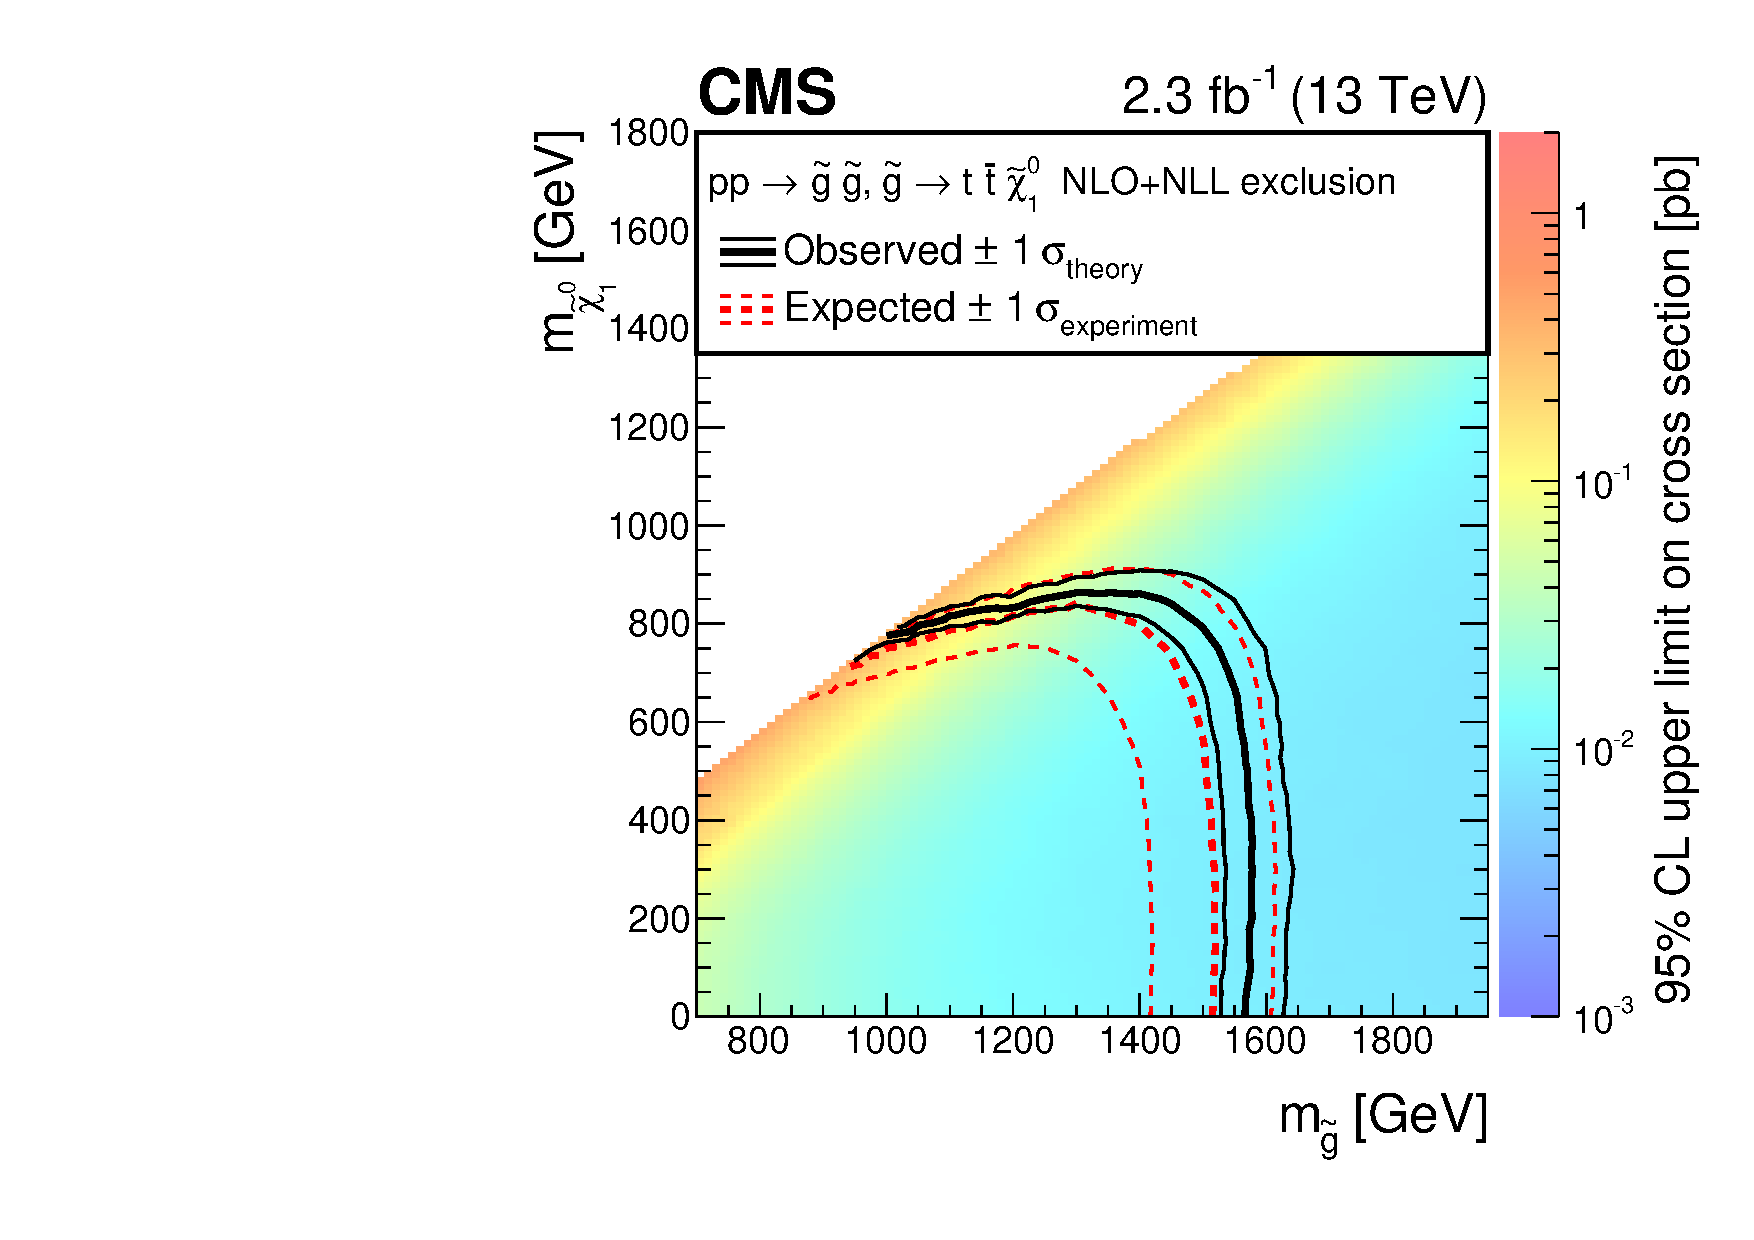
\includegraphics[width=0.45\textwidth]{Plots/analysis/results/CMS-SUS-15-006_Figure_007-a}
  \hfil
  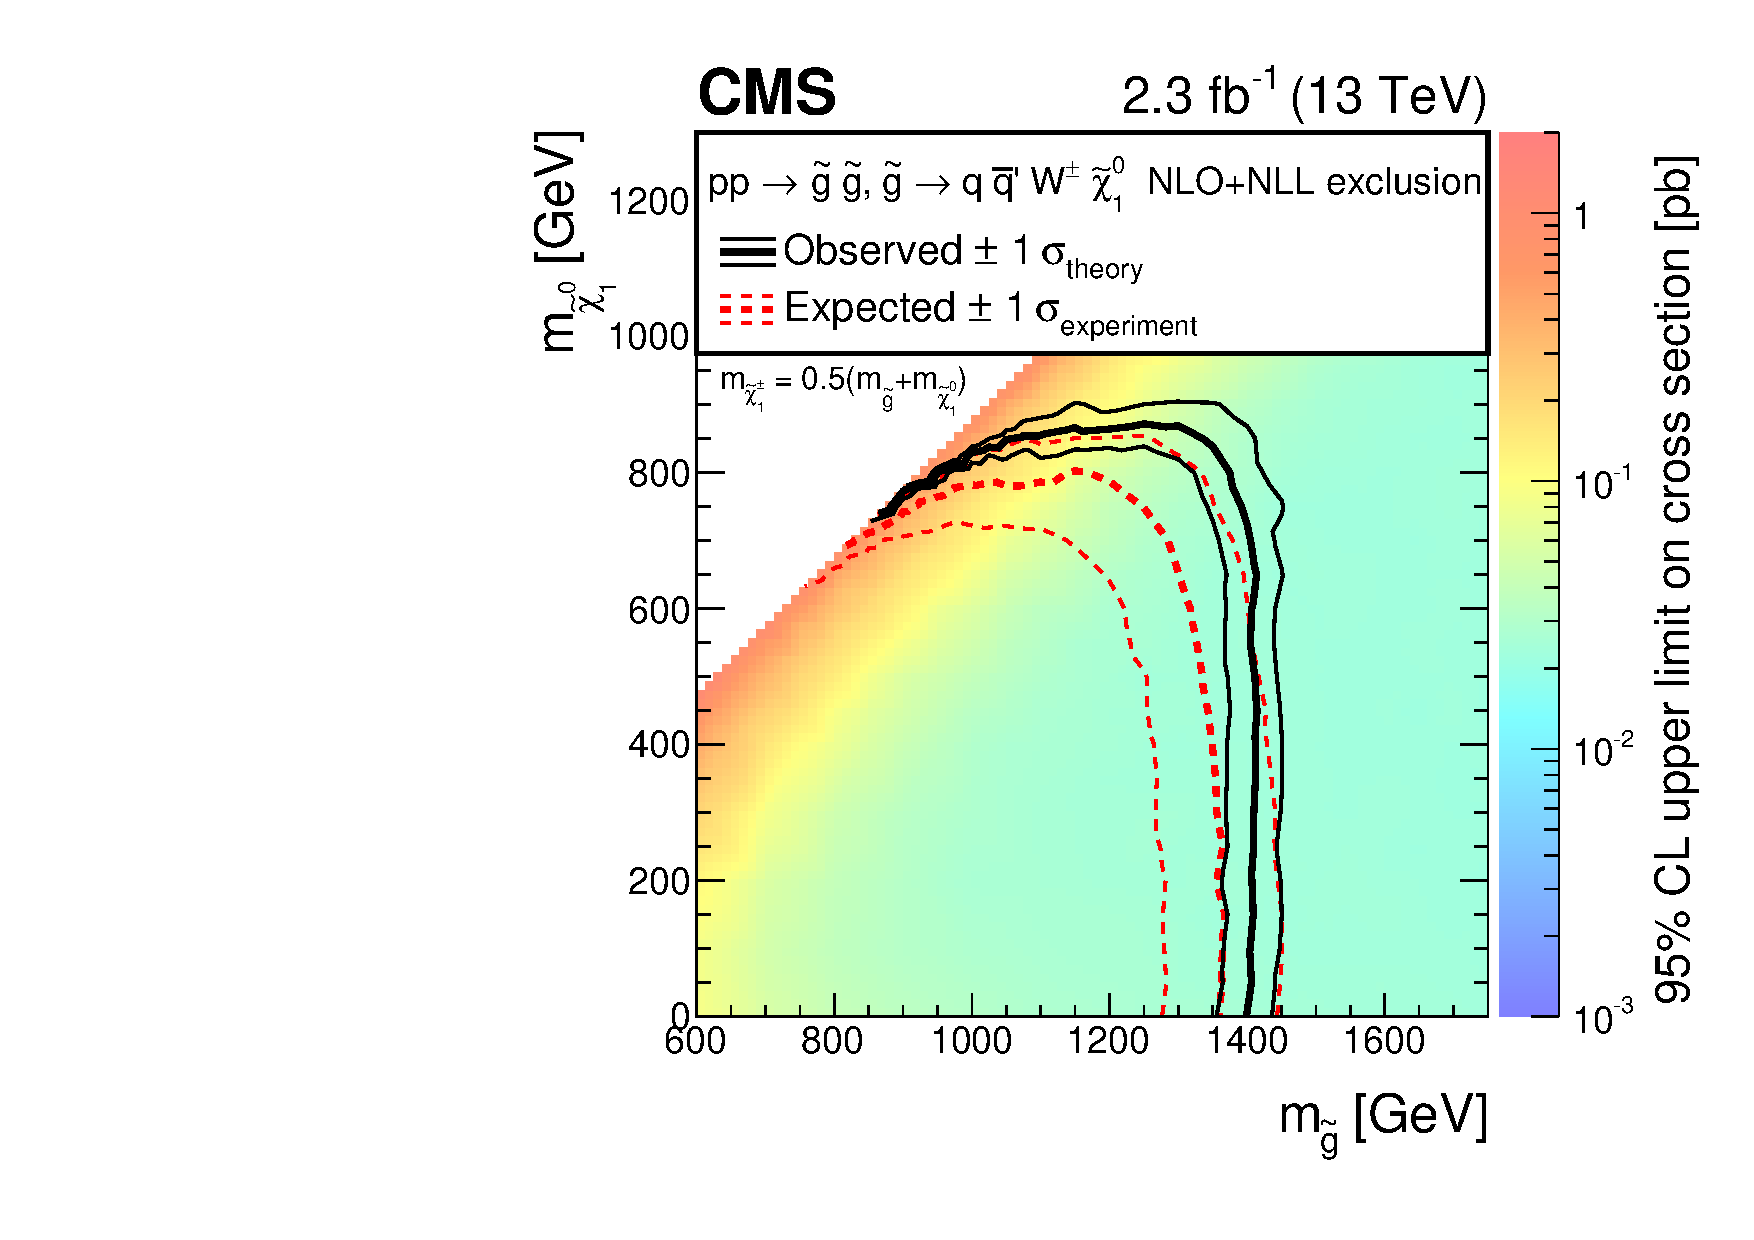
\includegraphics[width=0.45\textwidth]{Plots/analysis/results/CMS-SUS-15-006_Figure_007-b}
\centering
  \caption{\label{fig:Moriond} Cross section limits at a 95\% CL for (left) the T1tttt model, and (right) the T5qqqqWW model \cite{SUS_16_005}.
  }
\end{figure*}
\begin{figure*}[!hb]
\centering
  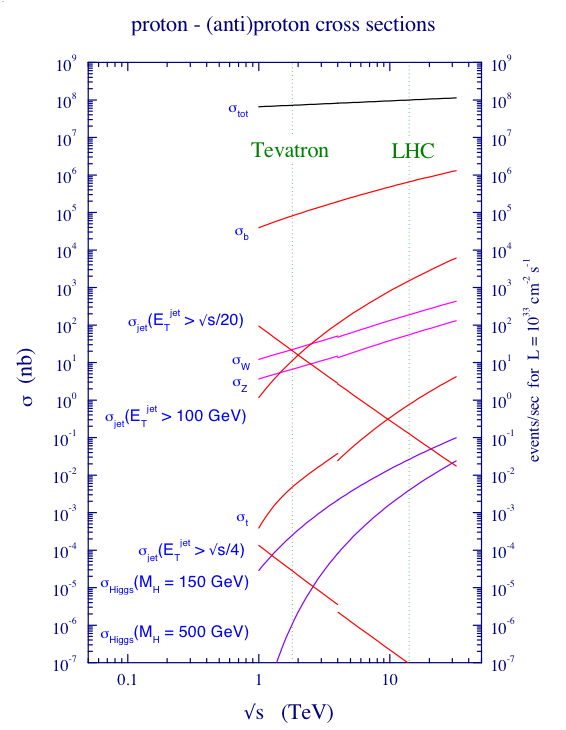
\includegraphics[width=0.7\textwidth]{Plots/SM/SMxsec}
  \caption{ Cross section of SM processes as a function of center of energy.
  ~\cite{smxsec}
  }
  \label{fig:sm_xsec}
\end{figure*}
%\newpage
%\lipsum
